\documentclass[11pt, a4paper]{article}
\usepackage[utf8]{inputenc}
\usepackage{mathpazo} % Palatino font
\usepackage{lineno}
\usepackage{setspace}
\usepackage{booktabs}
\usepackage{multirow}
\usepackage{caption}
\captionsetup{labelfont=bf}
\usepackage{graphicx, subcaption}
\usepackage{float}
\usepackage[margin=2cm]{geometry}
\usepackage{indentfirst}
\usepackage{natbib} 
\bibliographystyle{agsm}
\usepackage{amsmath}
\usepackage{tabularx}
\usepackage{siunitx}
\usepackage[version=3]{mhchem}
\usepackage{upgreek}
\usepackage{amssymb}
\usepackage{hyperref}
\usepackage[dvipsnames]{xcolor}
\hypersetup{
  colorlinks   = true, %Colours links instead of ugly boxes
  urlcolor     = blue, %Colour for external hyperlinks
  linkcolor    = black, %Colour of internal links
  citecolor   = black %Colour of citations
}

\newcommand{\reporttitle}{Influence of chemical and warming stressors on freshwater microbial function}
\newcommand{\reportauthor}{Chuxuan Ji}
\newcommand{\supervisor}{Guy Woodward}
\newcommand{\degreetype}{Master of Research}
\newcommand{\multiref}[2]{\autoref{#1}-\ref{#2}} % from - to

\begin{document}
\begin{spacing}{1.5}
\input{./titlepage.tex}


\section*{Declaration}
\addcontentsline{toc}{section}{Declaration}

I declare that the dissertation is my own work under the supervision of Prof. Guy Woodward. All sources of information are appropriately referenced. The Woodward lab group at Imperial College London established the mesocosm experimental protocols and design. The sampling of mesocosm was done by me with the assistance of some of the Woodward lab group members. Data for 2019 and 2021 are from previous raw data from Woodward lab. The work of lab trials, data sorting, calculation and statistical analysis is done by myself with the suggestion of my supervisor. No portion of the 2022 work referred to in the dissertation has been submitted in support of a degree or diploma or other qualification of this or any other university or other institute of learning. 

\clearpage

\section*{Abstract}
\addcontentsline{toc}{section}{Abstract}

Environmental stressors are ubiquitous in ecosystems, but the intricate effects of particular stressors on each other are challenging to assess. As one of the world's most endangered ecosystems, freshwater ecosystems are highly vulnerable to damage from human activities. Global warming and the widespread use of chemicals have led to very severe stresses on freshwater ecosystems. Yet most current research on freshwater microbes focuses on individuals or focal population responses that cannot capture the complexity of natural ecosystems. This study used 96 outdoor mesocosms to explore changes in freshwater microbial community function under pressure from biocides (four levels, four biocides representing each of urban and rural areas and their combinations) and gradient warming (nine levels, from ambient temperature to 8 °C warming). Half of the ponds (n=48) were treated with ammonia to explore the effects of organic pollution. The results showed that chemicals and warming significantly impacted BOD and litter decomposition. Chemicals exhibited significant non-additive effects among themselves and with temperature. This study did not find the effects of chemicals and warming on microbial ATP production and respiration, demonstrating the expected redundancy in microbial community function. Contrary to the expectations of this study, the results did not reveal any potential slope effects after comparing data from biocide-treated ponds from 2019-2022. This study shows how common freshwater microbial community functions change under chemicals and warming stress and provides ideas and new insights for future related research and policy development to address potential problems. 

\clearpage

\tableofcontents 
\clearpage

\linenumbers
\renewcommand\thesection{\arabic{section}}
\section{Introduction}

Freshwater ecosystems are among the most endangered globally and are particularly vulnerable to human activity \citep{dudgeon2006freshwater}, which is due to the disproportionately high biodiversity of freshwater ecosystems. For instance, freshwater habitats cover only 0.8\% of the Earth's surface but are home to one-third of the world's vertebrates and two-fifths of fish species \citep{lundberg2000so}. Due to human activities such as water pollution \citep{schwarzenbach2010global}, habitat destruction and degradation \citep{garrick2017valuing}, flow modification \citep{poff2007homogenization}, overexploitation \citep{malmqvist2002threats}, and invasion by exotic species \citep{rahel2002homogenization}, the biodiversity of already vulnerable freshwater habitats is dropping faster than that of the most contaminated terrestrial ecosystems \citep{sala2000global}. Also, freshwater is the most important natural resource after air \citep{qadri2020freshwater}, which can be exploited, controlled, or polluted at any time, leading to greater vulnerability of freshwater organisms. The rising contamination of freshwater systems worldwide is one of the biggest environmental challenges impacting humanity \citep{inyinbor2018water}. For geographical reasons, lakes and rivers are recipients of pollutants and sediments, but the volume of inland water bodies limits their ability to dilute them, which leads to greater damage to freshwater ecosystems \citep{dudgeon2006freshwater}. 

The main sources of freshwater pollution are domestic sewage \citep{hendriksen2019global}, industrial pollution \citep{ho2012industrial}, pharmaceuticals \citep{caracciolo2015pharmaceuticals}, and plastics \citep{blettler2019threats}. Among them, pharmaceuticals are critical to preserving public health and quality of life, including antibiotics, pesticides, herbicides, fungicides, etc. Every year, over 1.2 million tons of pesticides are used worldwide, affecting community structure and function in freshwater ecosystems \citep{gustavson2003effects, rohr2005effects, brovini2021three}. Due to the unregulated and misuse of biocides, almost more than half of them remain in the soil, and most of the rest of these biocides will enter the water, polluting the aquatic ecosystem \citep{babcock1992impact}. Many studies show that the biocides are not very hazardous to aquatic organisms because the pesticides currently in use have relatively short half-lives \citep{fantke2014estimating} and are usually present in natural water at reasonably low concentrations \citep{macherius2014triclocarban, santos2009occurrence}. While most biocides are intended to target specific species or groups of hazardous organisms, they often act on specific targets that are broadly conserved throughout many life forms and extend their effects to non-target species \citep{davidson2001declines}. On the other hand, Biocides are distinct from traditional pollutants in that they are expressly designed to be biologically active in low quantities \citep{garry2004pesticides}. Thus, biocides in freshwater have been linked to biodiversity loss as well as negative effects on ecosystems \citep{bridges2000long, horrigan2002sustainable}, and in some cases, the consequences of sublethal exposure to biocides on non-target animals have been discovered \citep{desneux2007sublethal, kurenbach2015sublethal, saravanan2011haematological}. Ammonia is widely present in the waters of developed countries as a major by-product of organic pollution \citep{abel2002water}. Urbanisation has significantly increased the ammonia concentration in groundwater and surface water, which has caused severe damage to freshwater ecosystems \citep{constable2003ecological,smith2003eutrophication}. Ammonia can alter cell pH \citep{zhang2018free}, break down extracellular polymeric substances and inhibit specific enzymatic reactions leading to cell death \citep{liu2019roles}. Low concentrations of ammonia can affect the movement, growth \citep{alonso2004toxic}, decomposition \citep{yenigun2013ammonia}, reproduction of aquatic organisms and even alter the composition of microbial communities \citep{zhang2020ammonia}.

In addition to pharmaceuticals, global warming is an anthropogenic stressor harming global freshwater biodiversity and ecosystems \citep{woodward2010climate}. Global temperatures will increase by 0.25-0.32 °C per decade in the short term \citep{smith2018predicted}, and this warming reduces 60\% of ecosystem services or social benefits \citep{mooney2009biodiversity} and will continue to lead to changes in ecosystem functioning over the next hundred years \citep{leducq2014local}. However, studies on the interaction between global warming and other anthropogenic stressors on freshwater organisms are complicated and may have synergistic (combined effect greater than individual effects) \citep{verberk2016field} or antagonistic effects (combined effect smaller than individual effects) \citep{jackson2016net}. The relationship between warming and chemicals shows the same phenomenon. On the one hand, the toxicity of some biocides increases when the temperature is increased \citep{jacobson2008combined, noyes2015forecasting}. On the other hand, the degradation rate of biocides such as pesticides and the solubility of ammonia increase and decrease with increasing temperature, leading to a reduction in the concentration of the chemicals \citep{kookana2010impact}. Meanwhile, biocides and ammonia can impair the ability of organisms to cope with rising temperatures \citep{hooper2013interactions, moe2013combined}. As a result, it is critical to investigate the impact of chemicals on freshwater ecosystems under rising temperatures and determine potential dangers.

Because of the intimate relationship with habitats \citep{falkowski2008microbial}, fast reaction to changing environmental conditions \citep{xue2016tundra}, and relatively high dispersion ability \citep{barberan2014microbial}, microorganisms are excellent predictors of ecosystem change. Humans can more reliably predict microbial functions and feedback mechanisms in response to environmental changes by investigating long-term microbial datasets \citep{buttigieg2018marine, saba2010challenges}. Microorganisms are vital degraders of organic matter and exogenous substances (including pharmaceuticals) \citep{paul2005accessing}, and can break down contaminants via metabolic and/or co-metabolic pathways \citep{caracciolo2015pharmaceuticals, topp2013accelerated}. Biocides and ammonia have complex effects on the structure and function of microbial communities \citep{melendez1993effects, widenfalk2004effects,zhang2020ammonia}. They primarily target their target organisms but may have broader harmful effects on microorganisms \citep{delorenzo2001toxicity}. For instance, oxytetracycline (an antibiotic) has been shown to inhibit the growth of some sensitive fungal species and reduce the length of active mycelium \citep{colinas1994population}. Tebuconazole (a fungicide) reduces the activity of dehydrogenases and thus affects bacterial degradation \citep{bending2007fungicide}, etc. Ammonia stress reduces antibiotic efflux from the interior of the bacteria but enhances antibiotic resistance \citep{zhang2020ammonia}. However, this makes partially biocide-tolerant microbial populations less competitive for shared resources \citep{johnsen2001pesticide}, increasing their growth and survivability. The majority of current research is on the microbial degradation of biocides rather than the impacts on natural microbial populations \citep{aislabie1995review, singh2006microbial}. Furthermore, research on the effects of chemicals on freshwater microorganisms is also fragmented, compared with far more studies on soil environments \citep{hussain2009impact, lupwayi2009changes}.

Freshwater ecosystems are frequently exposed to multiple stressors \citep{muturi2017effect}, and investigating microbial responses to these stressors may reveal changes in the function of freshwater microbial communities as well as changes in freshwater ecosystems. Most current studies investigating the effects of multiple anthropogenic stressors on microbial communities in freshwater ecosystems have focused on the effects of single species or pharmaceuticals or on simple 'before' and 'after' stress states \citep{bitton1992bacterial, downing2004effects, widenfalk2008effects}. Previous research has shown that multiple stressors are rarely fully synchronised in time and that the extent to which it affects organisms over time diminishes with multi-generational natural selection of organisms and species sorting due to past stresses, resulting in a slope effect \citep{gibert2015scaling,pawar2015metabolic,hughes2019ecological}. Meanwhile, non-additive responses to multiple stressors affect the actual outcome of climate change \citep{woodward2010climate}, and ecosystem-level mesocosm experiments can most directly predict the ecological impact of such changes \citep{feuchtmayr2009global}. This study used mesocosm experiments to quantify the effects of mixtures of biocides representing three typical environments (URBAN, RURAL and UR+RU), organic pollution (ammonia), and gradient warming (from ambient temperature to ambient + 8°C) on freshwater microbial communities under sub-lethal concentrations of chemical and warming stresses. 4°C temperature difference matched the predicted 4°C increase in ambient temperature by 2100 under RCP 8.5 \citep{stocker2014climate}. Here this study test the hypothesis that chemical mixtures and warming cause changes in freshwater microbial community functions and address the following questions: (1) \textit{Are there non-additive interactions between chemicals and with warming?} (2) \textit{Is there redundancy in community function due to the high taxonomic diversity of microbial communities?} (3) \textit{Does microbial community function exhibit a ramping effect after sustained biocide exposure?} 

\section{Material and Methods}

\subsection{Experimental mesocosms}

The mesocosm experiments are carried out in the Silwood Park pond mesocosm sited in southern England (Imperial College London Silwood Park campus, Ascot, SU 93790 69372). Experiments were conducted in artificial tanks approximately 2m in diameter and 1m deep that could hold 1800L of fresh water. The ponds were filled with sand/gravel from Silwood Lake (March 2016) and a combination of water, sediment, and biota from adjacent water bodies (outflow streams, lakes, etc.), followed by natural colonization. This "open system" allows the ponds to receive organic matter and natural exposure and therefore supports a realistic level of biological complexity, which is ideal for experimenting at the community level and exploring the effects of environmental change at the ecosystem level \citep{stewart2013mesocosm}.  

To simulate global warming, a selection of these ponds (n=96) began to be continuously warmed by 1°C to 8°C above ambient temperature beginning in 2018. Meanwhile, from 2018 through 2022, a subset of 32 ponds got dosed with biocide mixtures every three months. Each biocide is widely used in the UK and targets specific portions of the food web/taxa group, assuring their widespread existence and different mechanisms of action in UK freshwater ecosystems. To investigate the impact of organic contamination, ammonia was dosed on half of the ponds (n=48) from 2021 (Figure \ref{fig:Mesocosm} and Table \ref{tab:Treatment}).

Here, six different treatments were selected for analysis: undisturbed ambient conditions (CONTROL), 4°C warming (4°C), urban biocide mix (URBAN), rural biocide mix (RURAL), urban and rural biocide mix (UR+RU) and urban and rural biocide mix + 4°C warming (UR+RU+4°C). These treatments were used to explore the effects of biocide mixes in different use environments (urban and rural) and elevated temperatures on the freshwater microbial community. The composition of the biocide mixes representing the different environments is shown in Table \ref{tab:Biocide}, each containing one each of an herbicide, pesticide, fungicide, and antibiotic.

\begin{table}[H]
    \caption{\bf Biocide treatments used in the current study.}
    \centering
    \begin{tabular}{ |m{2.5cm}<{\centering}|m{3cm}<{\centering}|m{2cm}<{\centering}|m{7.5cm}<{\centering}| } 
    \hline
     Biocide Mix & Biocides & Type & Mode of action \\
     \hline
     \multirow{4}*{URBAN} & Glyphosate & Herbicide & Inhibiting EPSP synthase \\ 
     & Imidacloprid & Pesticide & Blocking the nicotinergic neuronal pathway \\
     & Tebuconazole & Fungicide & Inhibiting the biosynthesis of ergosterol to disrupt fungal cell membranes \\
     & Amoxicillin & Antibiotic & Inhibiting transpeptidation, leading to cell wall cleavage \\
     \hline
     \multirow{4}*{RURAL}& Diflufenican & Herbicide & Inhibiting the biosynthesis of carotenoids \\
     & Metaldehyde & Pesticide & Limiting mucus production in molluscs \\
     & Chlorothalonil & Fungicide & Inhibiting fungal spore germination, glycolysis, and fungal respiration \\
     & Oxytetracycline & Antibiotic & Inhibiting translation to inhibit cell growth \\
    \hline
    \end{tabular}    
    \label{tab:Biocide}
\end{table}

\subsection{Sampling methods}

Samples were taken within 14-18 days before and after each dosing event. When taking water samples, use a 100ml dipper to transfer 200ml of water from the middle and four directions (N.S.E.W) to a 1.6L Whirl-Pak$^\circledR$ bags. A 50 ml water sample was then drawn from the middle of the pond using a 50 ml serological pipette and transferred to a 50 ml centrifuge tube. Finally, a 500ml water sample was taken in the middle of the pond using a 500ml Nalgene$^\circledR$ bottle. For sediment samples, transfer 10 ml sediment samples to 50 ml centrifuge tubes using a 50 ml serological pipette in the pond's middle and three orientations (N.S.W).

\subsection{Microbial functioning assays}

\begin{figure}[H]
    \centering
    \includegraphics[scale=0.83]{./Figures/WorkFlow}
    \caption{\textbf{Schematic of experimental ponds set-up and microbial function measurements.} Water and sediment samples were taken in mesocosm ponds (A) 14-18 days before and after dosing. After sampling, ATP production from sediment wash, sediment, and water samples was measured (B). The number of cells in the water samples was recorded by flow cytometer (C) to calculate each cell's production. Sediment wash samples were used to measure microbial respiration using the MicroResp$^\text{TM}$ system (D). Water samples collected in Nalgene bottles were tested for dissolved oxygen on the same day and measured again five days later to calculate $BOD_5$ (E). Coarse and fine leaf bags and two types of tea bags were placed in the pond for 32 days to measure decomposition (F). For further details on the mesocosm and microbial functional analysis, see Figure \ref{fig:Mesocosm} and Section \ref{section:M_ATP}-\ref{section:M_Decomposition}.}
    \label{fig:WorkFlow}
\end{figure}

In this study, microbial ATP assays, MicroResp$^\text{TM}$, biochemical oxygen demand ($BOD_5$), decomposition (leaf, tea bags and Wettex$^\circledR$) and microbial enzyme assays were carried out, and cell counts in the water samples were calculated by flow cytometry (Figure \ref{fig:WorkFlow}. Among these, the enzyme assay was discarded for the spring 2022 post-dosing as enzyme assays in 2019 and 2021 did not demonstrate biocide and warming effects. The result of Wettex decomposition was also removed due to having lots of outliers. The analysis of the enzyme assay for spring 2019 to spring 2022 pre-dosing and Wettex$^\circledR$ decomposition is conducted in the supplementary (Section \ref{section:Enzyme} and \ref{section:Wettex}). 

For water samples, 2 ml of water was pipetted from each 50 ml water sample centrifuge tube into a 2.2 ml deep 96-well plate. For sediment samples, the centrifuge tubes were placed on a platform shaker to shake the samples at 250 rpm for 10 minutes and then left to stand for another 10 minutes. Afterwards, 2 ml of sediment wash was pipetted into the deep well plate using a wide orifice tip at the interface of water and sediment. The supernatant was then poured off, the remaining sediment was mixed again, and 2 ml of sediment was aspirated into the deep well plate. The remaining sediment was dried for 24h and weighed. Two deep-well plates of each type were made, one will be frozen at 80°C as a spare, and the other will be used for microbial functional assays. 

\subsubsection{ATP assay}\label{section:M_ATP}

Water, sediment wash and sediment ATP were measured in this study. The sediment samples were diluted at 1:50. 98$\upmu$l of PBS and 2$\upmu$l of the samples were added to a white 96-well plate and placed in a BioTek$^\circledR$ Synergy 2 Multi-Detection Microplate Reader. BioTek$^\circledR$ Synergy 2 Reader dispensed 25$\upmu$l of BacTiter-Glo Reagent into each well, then read luminescence every 1min15s for 5 minutes after a medium shake for 5s. ATP (nmol $g^{-1}$) can be computed from maximal luminescence using the following equation:

\begin{align}\label{eq:ATP}
    \operatorname{ATP\ (nmol\ g^{-1})} = {\left(\operatorname{Lum\ of\ sample} - \operatorname{Lum\ of\  control} / 1693.1 \right)\times \operatorname{dilution\ factor}}
\end{align}

\subsubsection{Flow cytometer}\label{section:M_Flow}

In this study, microbial abundance was recorded only in water samples. 198$\upmu$l of 1:10 diluted water sample and 2$\upmu$l of 1:1000 diluted thiazole orange solution was added to a 96-well plate. On the BD Accuri$^\text{TM}$ C6 Software, set the running limit of Fast Fluidics to 10$\upmu$l and set the ESC-H threshold to 8000 to exclude small particulate matter. Cell counts were subsequently performed on the BD Accuri$^\text{TM}$ C6 flow cytometer.

\subsubsection{MicroResp$^\text{TM}$}\label{section:M_MR}

In this study, the MicroResp$^\text{TM}$ system was used to measure the respiration of the microbial community of the sediment wash \citep{campbell2003rapid}. First, 1.875mg cresol red, 1.677g \ce{KCl} and 0.0315g \ce{Na2CO3} were added to 100ml deionized water to make an indicator. Afterwards, a 3\% agar solution was prepared and autoclaved. The indicator was added when the agar was cooled to 60°C, and the mixture was transferred to 150$\upmu$l of the 96-well plate. The agar solidified plates were placed in a dry box with soda lime for 24 hours and then read at 570 nm. 500$\upmu$l sediment wash was transferred to 96 deep well plate, and the agar-treated 96-well plate was fixed on both sides of the MicroResp$^\text{TM}$ Seal and clamped. Bacterial respiration was measured on the third and seventh days by BioTek$^\circledR$ Synergy 2 Reader, respectively. CO2 (mg) evolved from carbon substrate utilisation was then computed from $\upDelta \uplambda 570$ (difference in absorbance (570nm) at start and end) using the following equation \citep{rivett2016resource}:

\begin{align}\label{eq:MicroResp}
    \operatorname{\ce{CO2}\ (mg)} = e^{\left((ln(\upDelta \uplambda570) + 0.305414) / 0.282164 \right)}
\end{align}

\subsubsection{Biochemical Oxygen Demand (BOD)}\label{section:M_BOD}

Biochemical Oxygen Demand (BOD) was measured on the day and five days after sampling. After filling the sterilized Environmental Express$^\circledR$ BOD bottles with the collected water sample, use HAILEA$^\circledR$ super silent adjustable air pump ACO-9630 to inflate for 15 minutes and then use HANNA$^\circledR$ HI-5421 Research Grade DO \& BOD Bench Meter for BOD according to the manufacturer's instructions to measure. They were then stored in the dark at 20°C in a climate-controlled room for five days and measured again.

\subsubsection{Decomposition}\label{section:M_Decomposition}

Measuring ecosystem functioning, such as decomposition rates, may be a more sensitive predictor of the impact of anthropogenic pressure on ecosystems than community structure \citep{gessner2002case}. This study employs three methods that measure decomposition representing decomposers from different organisational levels in the ecosystem: leaf litter and tea bag decomposition. Also in this study the decomposition of Wettex$^\circledR$ was analysed, which is explained in detail in the supplementary (Section \ref{section:Wettex}), however the result was removed due to having lots of outliers. At the same time, the decomposition rates of the three materials utilised are also different due to differences in carbon content and tensile strength, which makes the measurement of this ecosystem function more objective. The decomposition rate (\textit{k}) was calculated using the following equation:

\begin{align}\label{eq:Decomposition}
    \frac{m_t}{m_0} = e^{-kt}
\end{align}
where $m_t$ is the measured dry weight after incubation time \textit{t} and $m_0$ is the start dry weight. In order to correct for potential temperature differences between ponds, in this study \textit{t} is also expressed in thermal sums (degree-days).

In this study, dried alder (\textit{Alnus glutinosa}) leaf litter collected every autumn was weighed to 1.5 g and rehydrated with deionised water to prevent breakage. The leaves were packed into two mesh bags with 10 mm and 500 um mesh apertures to investigate the total and microbial decomposition. The leaves were dried in an oven for 48h at 60°C before incubating. After 32 days of culture in mesocosms, the leaf litter bags were taken out, then first rinsed with deionised water, and re-weighed (±0.01 g) after drying. The leaf litter loss is calculated by subtracting the ending weight from the starting weight.

The degree of decomposition of the two tea bags with contrasting decomposition was used in this study as another standardised indicator of decomposition \citep{keuskamp2013tea}; the green tea (\textit{Camellia sinensis}; Lipton$^\circledR$, \copyright Unilever; EAN: 8 722700 055525), and rooibos tea (\textit{Aspalanthus linearis}; Lipton$^\circledR$, \copyright Unilever; EAN: 8 722700 188438). The start weights of the tea in the tea bags were measured at the beginning (tea bag dry weight - empty bag weight), followed by incubation in mesocosms for 32 days. At the end of the incubation, the tea bags' dry weight was dried in an oven at 60°C for 48h. The tea bags were then weighed, and the decomposition rate was calculated.

\subsection{Statistical analyses}

This study used a linear mixed-effect model (LMM) to examine differences in microbial function (ATP, respiration, BOD and decomposition) between the control and the treatments (chemicals and warming). The chemicals and warming treatments were used as fixed factors at four and nine levels. Ponds were used as random factors to account for potential differences between ponds. Significance levels were determined based on p-values < 0.05, and the corresponding standardised effect sizes (Cohen's d) were calculated \citep{cohen2013statistical}. For the warming treatments, simple regression analysis was used to determine the change in microbial function with temperature.

All statistical analyses and visualisations were performed in the R (v.4.1.0) statistical environment \citep{ihaka1996r}. All LMMs were fitted using the R package "lmerTest" \citep{kuznetsova2017lmertest}. After determining the best-fit models, Cohen's d values were calculated using the 'EMAtools' package \citep{kleiman2017ematools}. Pearson correlation coefficients and trend lines for simple regression equations were derived from the 'ggpubr' package \citep{kassambara2020package}.

\section{Results}

\subsection{Freshwater microbial responses to multiple stressors (chemicals and warming) in 2022}

\subsubsection{ATP production}

\begin{figure}[H]
    \centering
    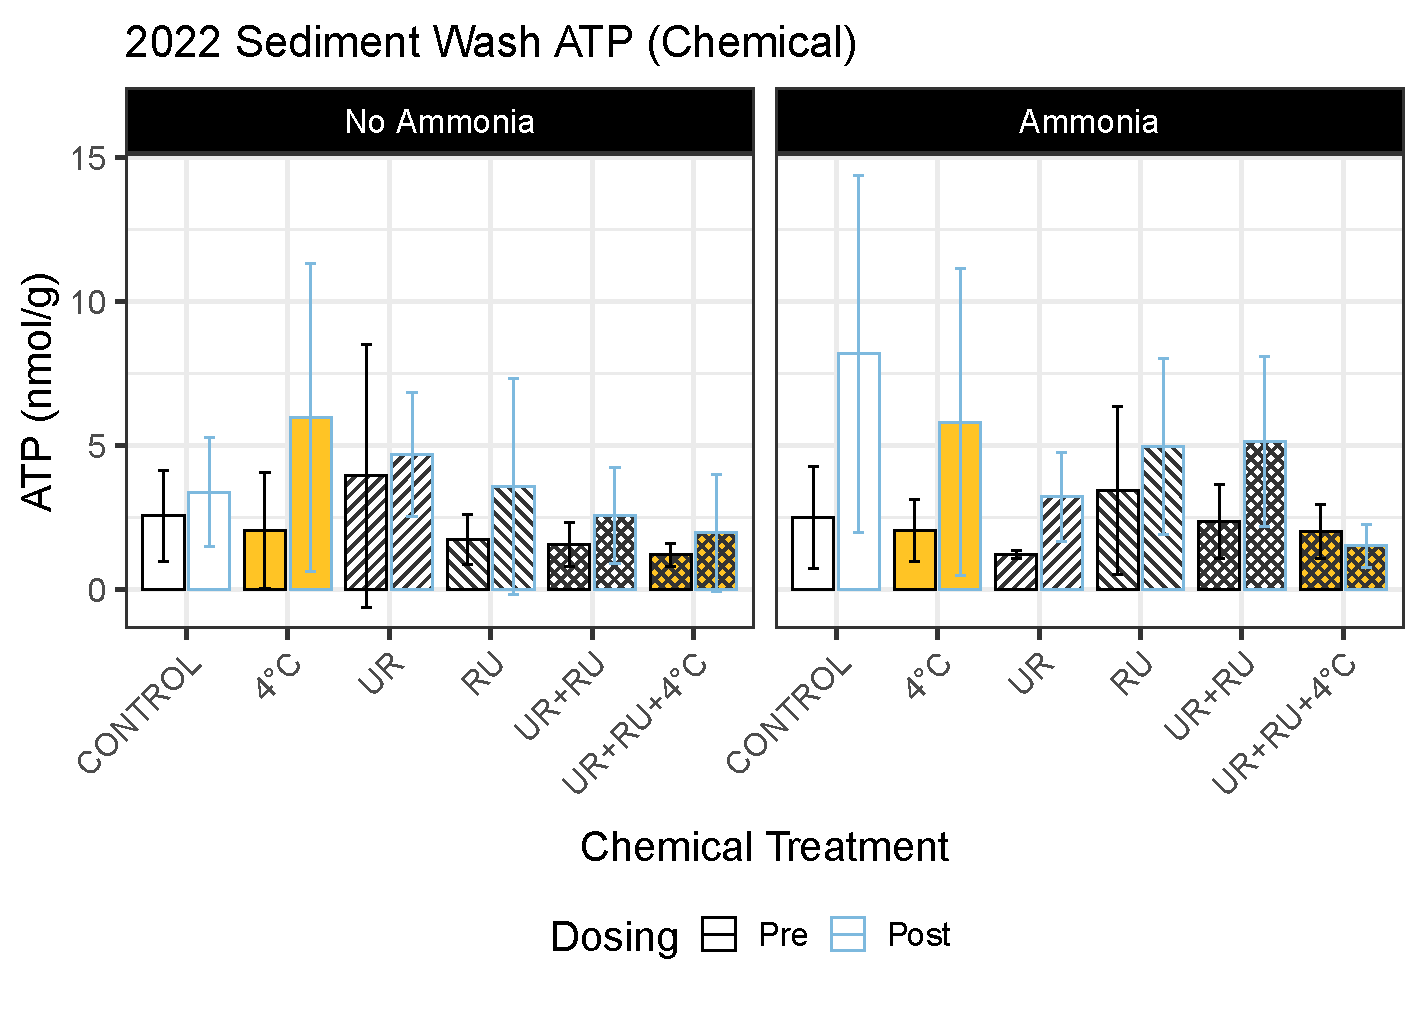
\includegraphics[scale=0.55]{./Figures/ATPSW2022_bar_chem}
    \caption{\textbf{Effects of chemicals on microbial ATP production in 2022.}UR represents the URBAN chemicals group and RU represents the RURAL chemicals group. Half of the 96 ponds were treated with ammonia. Biocides and warming showed a synergistic effect and reduced the production of ATP. }
    \label{fig:ATPSW2022_cp}
\end{figure}

All chemical groups and gradient warming had no significant effect on microbial ATP production after dosing (Table \ref{tab:ATPSW_treat}). UR+RU showed a coordinated effect; however, the two chemical groups showed a non-additive impact on the ammonia-treated ponds (Figure \ref{fig:ATPSW2022_cp}). The combination of warming and the two chemical groups (UR+RU+4°C) showed a synergistic effect. Regression analysis showed that temperature did not explain microbial ATP production in the warming ponds (Figure \ref{fig:ATP2022Regression}). In the warming-treated ponds, only the ammonia-treated 5°C warming significantly affected ATP production (Table \ref{tab:ATPSW_temp}, Figure \ref{fig:ATPSW2022_temp}), and in a positive direction.

\begin{figure}[H]
    \centering
    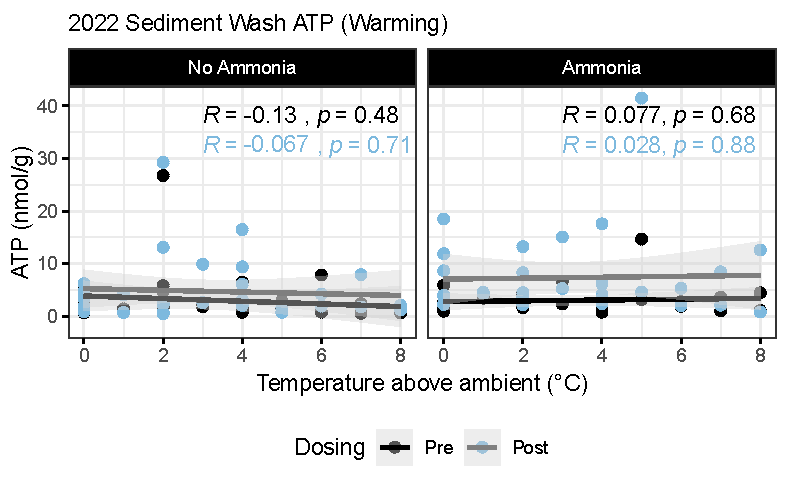
\includegraphics[scale=1]{./Figures/Regression_ATPSW}
    \caption{\textbf{Trends in ATP production with warming in 2022 for samples from sediment wash.} Gradient warming did not affect ATP production significantly.}
    \label{fig:ATPSW2022Regression}
\end{figure}

\subsubsection{Microbial respiration}

\begin{figure}[H]
    \centering
    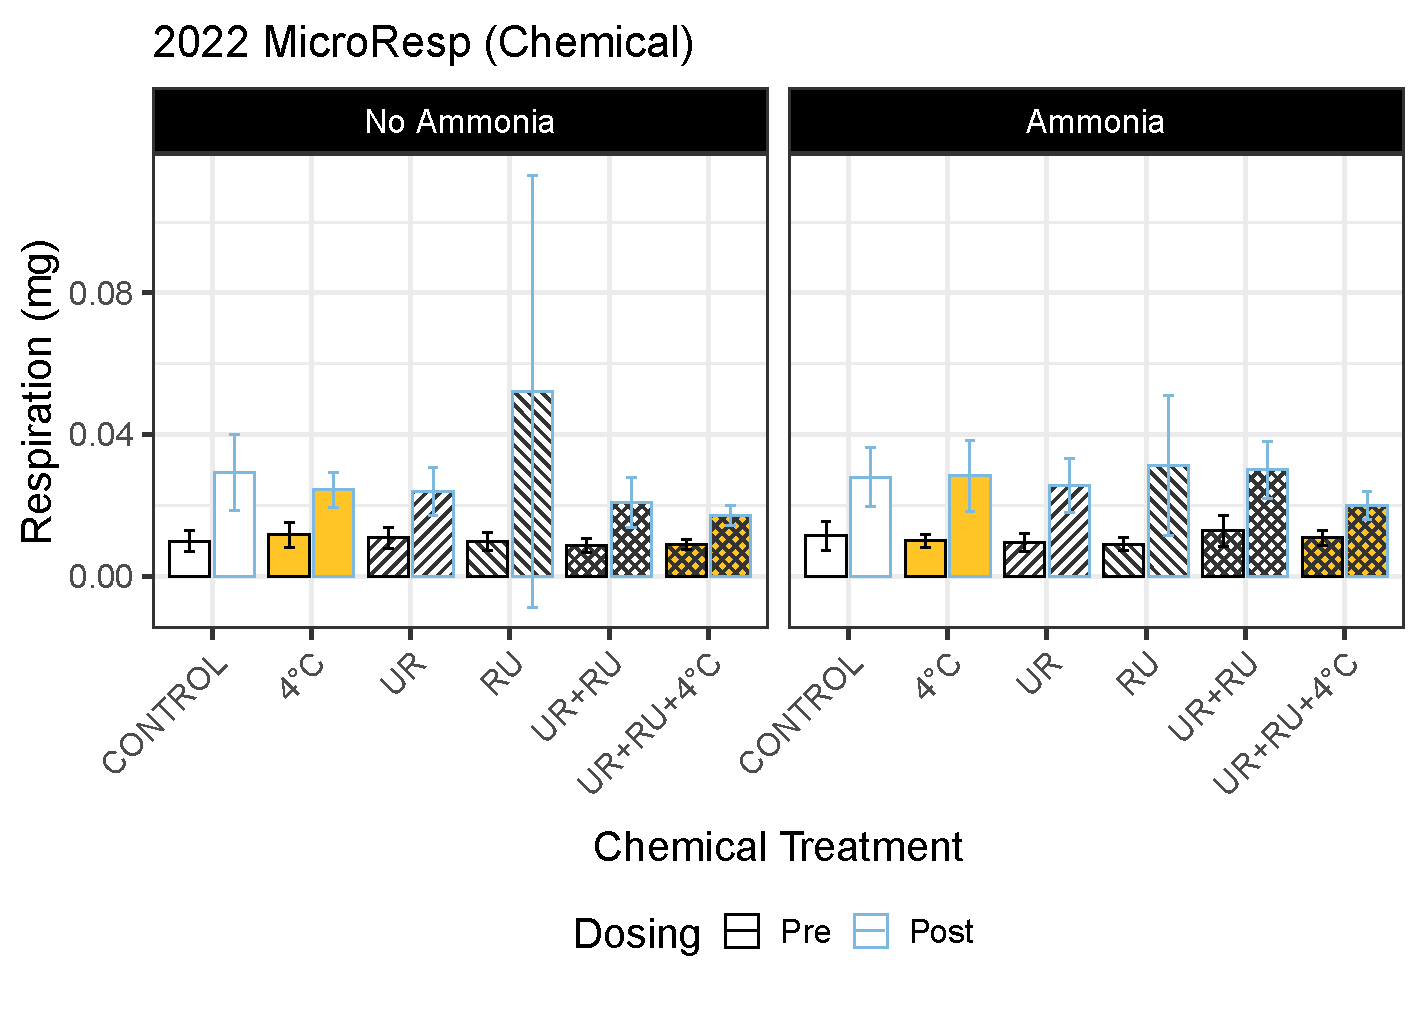
\includegraphics[scale=0.55]{./Figures/MicroResp2022_bar_chem}
    \caption{\textbf{Effects of chemicals on microbial respiration in 2022.} Ammonia has antagonistic effects with chemicals. The combination of warming (4°C) and chemicals synergistically reduced microbial respiration.}
    \label{fig:MicroResp2022cp}
\end{figure}

The linear mixed model showed that chemical and warming treatments did not affect microbial respiration (Table \ref{tab:MR_treat}). The combination of warming (4°C) and the two chemical groups produced a synergistic effect and reduced microbial respiration, whereas the chemical treatments at ambient temperature did not show any significant impact (Figure \ref{fig:MicroResp2022cp}). Likewise, regression analysis showed that warming did not explain the change in respiration (Figure \ref{fig:MR2022Regression}). There were no outliers in the warming-treated ponds (Table \ref{tab:MR_temp}, Figure \ref{fig:MR2022_temp}).

\begin{figure}[H]
    \centering
    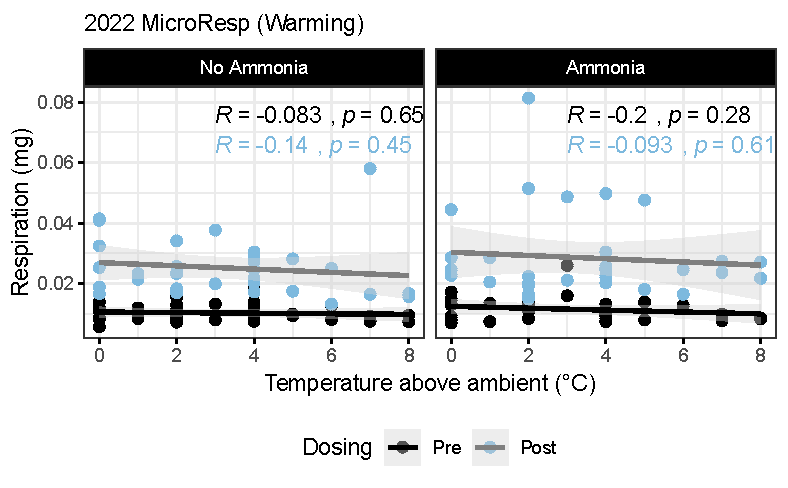
\includegraphics[scale=1]{./Figures/Regression_MicroResp}
    \caption{\textbf{Trends in microbial respiration with warming in 2022.} Gradient warming did not affect respiration significantly.}
    \label{fig:MR2022Regression}
\end{figure}

\subsubsection{Biochemical oxygen demand analysis}

\begin{figure}[H]
    \centering
    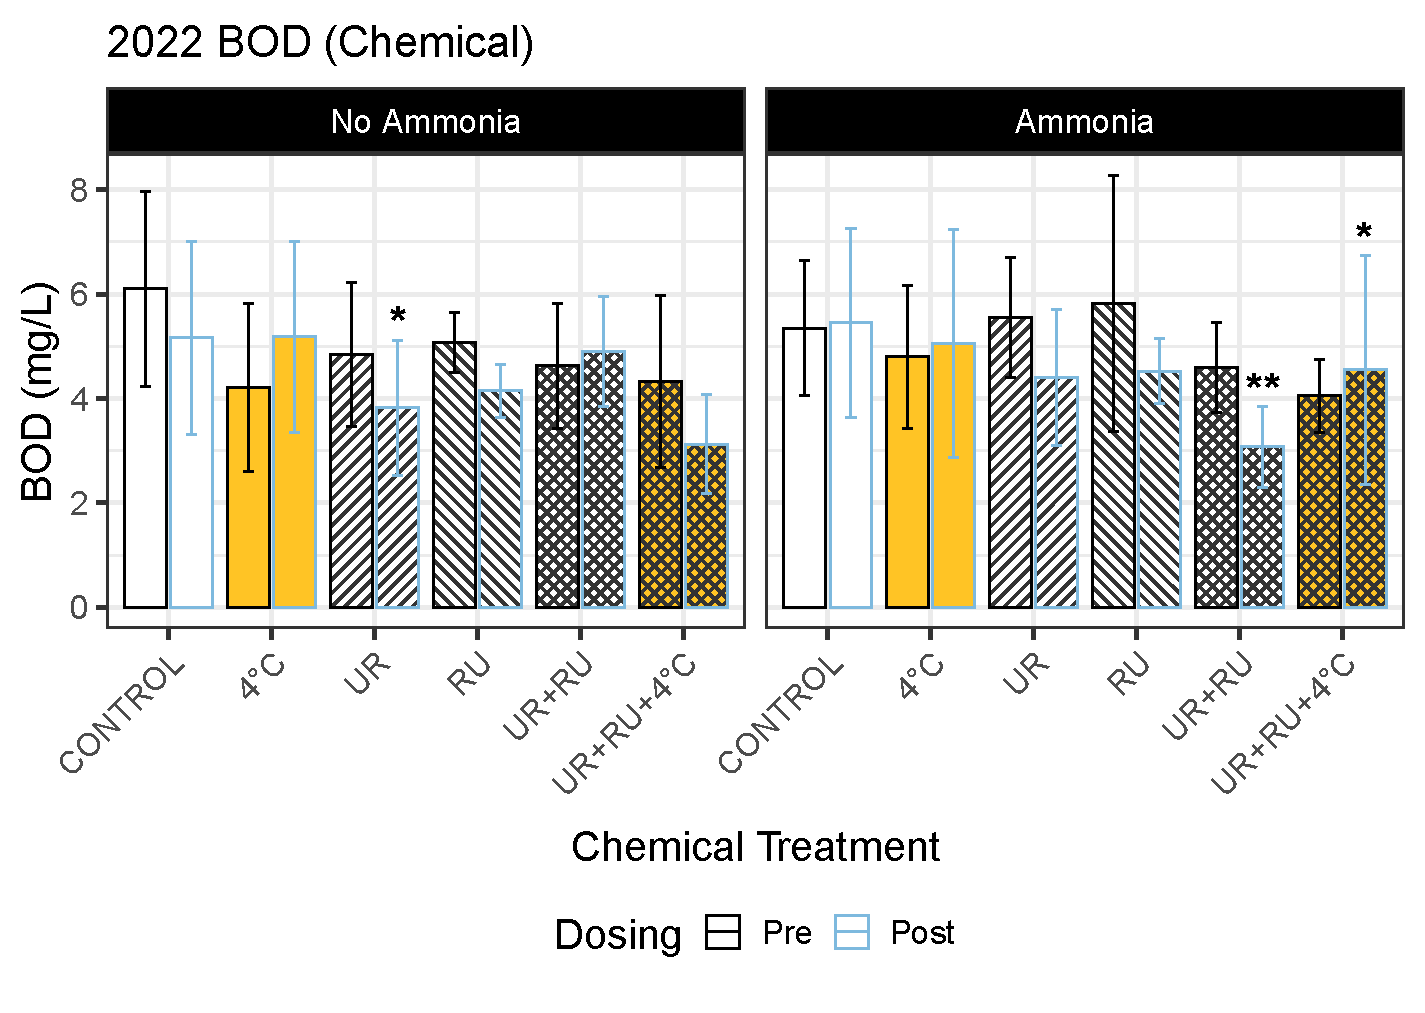
\includegraphics[scale=0.55]{./Figures/BOD2022_bar_chem}
    \caption{\textbf{Effects of chemicals on biochemical oxygen demand in 2022.} The combination of the two chemical groups and the combination of them and warming (4°C) showed opposite effects on BOD in the ponds with and without ammonia treatment.}
    \label{fig:BOD2022cp}
\end{figure}

Only URBAN chemicals group had a significant negative effect on BOD after dosing (Table \ref{tab:BOD_treat}). In the ammonia-treated ponds, UR+RU had a significant and negative impact on BOD. However, they had a significant antagonistic effect with warming (4°C) and increased BOD significantly. The two chemical groups continued to show a non-additive effect. At the same time, UR+RU+4°C significantly reduced BOD (Figure \ref{fig:BOD2022cp}). Still, the opposite was confirmed in the ammonia-treated ponds, where the two chemical groups showed a synergistic effect, and UR+RU+4°C showed a non-additive effect. Again warming did not significantly affect BOD, which was confirmed in the regression analysis (Figure \ref{fig:BOD2022Regression}). There were no outliers in the warming-treated ponds (Table \ref{tab:BOD_temp}, Figure \ref{fig:BOD2022_temp}).

\begin{figure}[H]
    \centering
    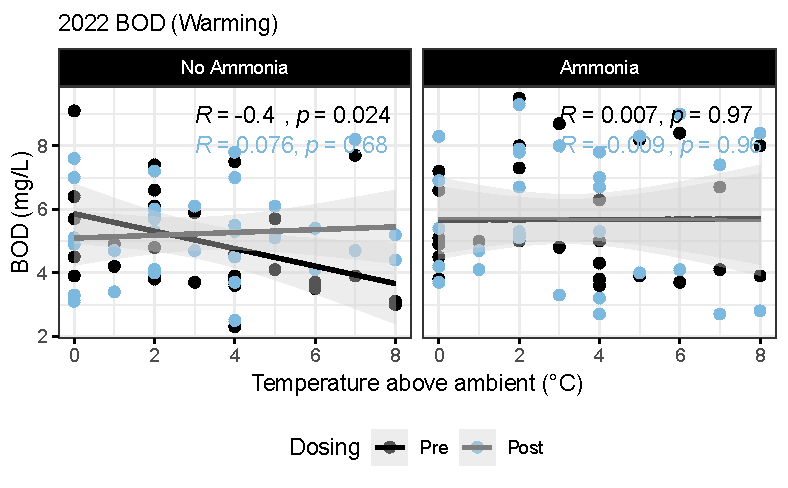
\includegraphics[scale=1]{./Figures/Regression_BOD}
    \caption{\textbf{Trends in BOD with warming in 2022.} Before dosing, the BOD of ponds without ammonia decreased with increasing temperature. After dosing, warming did not affect BOD significantly.}
    \label{fig:BOD2022Regression}
\end{figure}

\subsubsection{Decomposition analysis}

After dosing, the URBAN and RURAL chemical groups significantly affected the decomposition of rooibos tea bags in ammonia-treated ponds, with negative and positive effects, respectively (Table \ref{tab:D_2022chem}). While the decomposition rate of green tea was significantly elevated by the stress of UR+RU+4°C. After temperature correction, the URBAN chemicals group significantly reduced the decomposition of tea bags in the ammonia-treated ponds, and the RURAL chemicals group significantly reduced green tea decomposition rate in the ammonia-treated ponds. UR+RU significantly decreased the decomposition rate of green tea. In contrast, UR+RU+4°C significantly increased the rates for all decomposition but rooibos tea in the ammonia-treated ponds. Also, UR+RU+4°C  showed a positive impact, as did RURAL chemicals treatment on rooibos tea, the rest being all negative directions of significant effects. As Figure \ref{fig:Tea2022ccp} shown, all but UR+RU+4°C reduced the decomposition rate after correction for temperature. The combination of RURAL and URBAN chemical groups had non-additive effects on decomposition . Whereas there were non-additive effects between warming and chemicals before temperature correction, synergistic effects were shown after correction.

\begin{figure}[H]
    \centering
    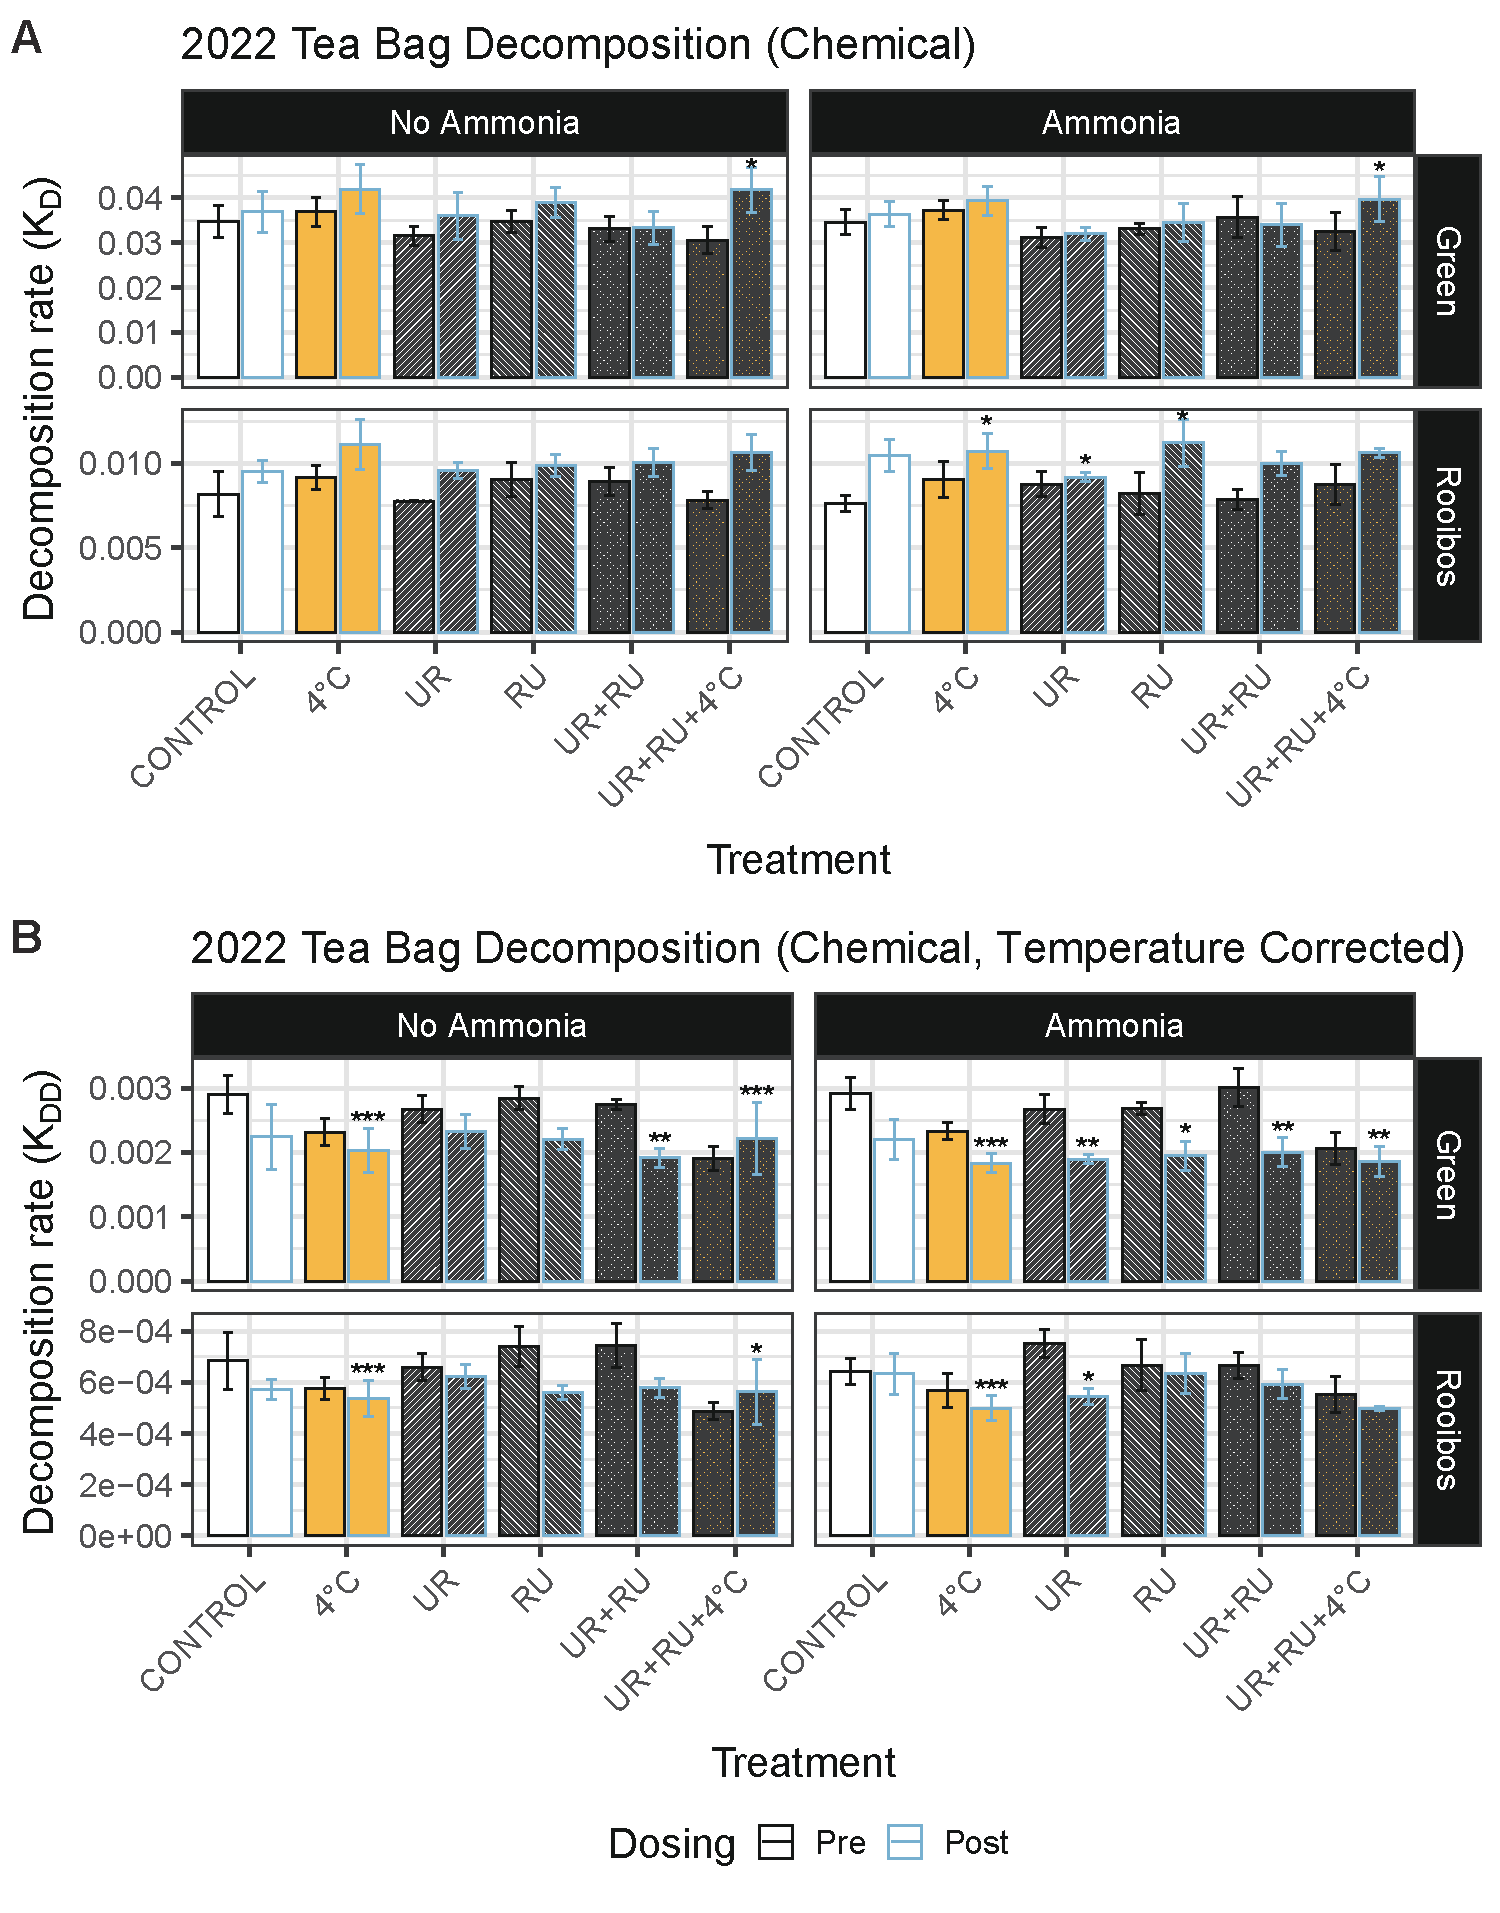
\includegraphics[scale=0.55]{./Figures/Tea2022_Treat_bar}
    \caption{\textbf{Effects of chemicals on tea bag decomposition in 2022.} The decomposition of green tea bags showed an antagonistic effect between the two chemical groups, except in green tea bags from ponds that had not been treated with ammonia. And UR+RU+4°C did not significantly alter the rate of decomposition. The increasing temperature increased the decomposition rate, while after temperature correction, the temperature decreased it.}
    \label{fig:Tea2022ccp}
\end{figure}

Regression analysis showed that increasing temperature increased decomposition rates in the ponds without ammonia treatment (Figure \ref{fig:Tea2022Regression}). In contrast, the effect of temperature on decomposition rates in the ammonia-treated ponds was insignificant. After temperature correction, temperature explained the decomposition of both kinds of tea bags in all ponds, and the decomposition rate decreased with increasing temperature. The specific effect of each temperature on the decomposition rate is shown in Table \ref{tab:D_2022temp} and Figure \ref{fig:Tea2022tcp}.

\begin{figure}[H]
    \centering
    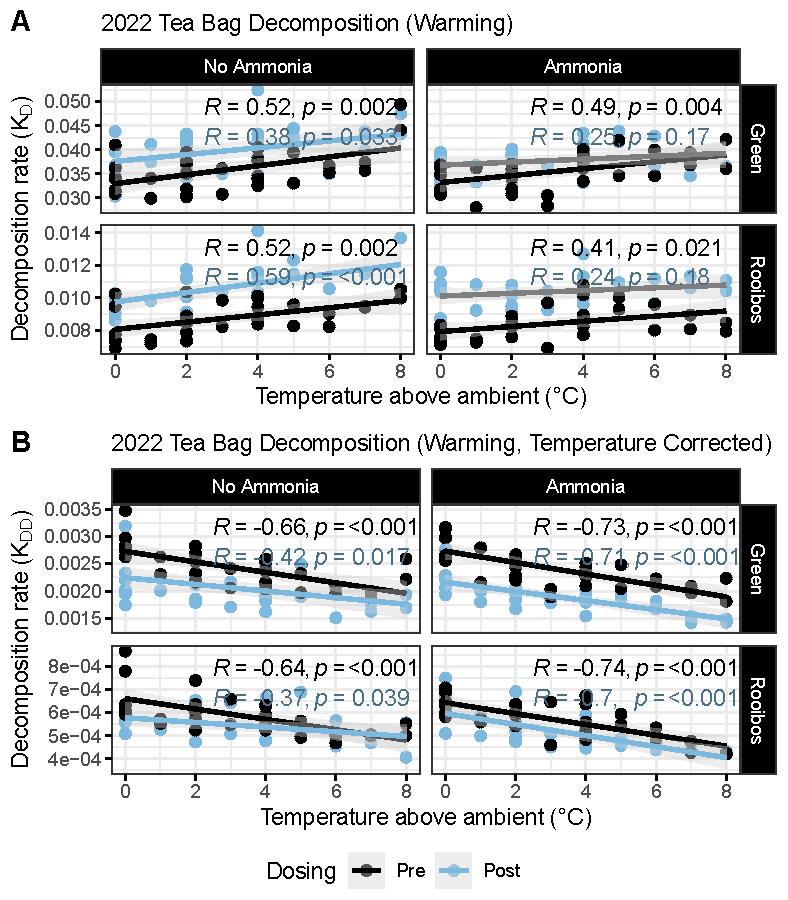
\includegraphics[scale=1]{./Figures/Regression_Tea}
    \caption{\textbf{Trends in tea bag decomposition rates with warming in 2022.} The decomposition rates were all significantly correlated with gradient warming before dosing. After dosing, decomposition rate increased with increasing temperature in ponds without ammonia treatment. After temperature correction, the rate of decomposition decreased with increasing temperature. The rate of decomposition decreased more rapidly in the ammonia-treated ponds.}
    \label{fig:Tea2022Regression}
\end{figure}

\subsection{Freshwater microbial responses to chemical stressors 2019 to 2022}

\subsubsection{ATP production}

The LMM showed that UR+RU significantly reduced ATP production over three years, while the other treatments had no significant effect (Table \ref{tab:ATPSW_3Year}). In 2021 and 2022, the URBAN and RURAL chemical groups had a highly significant synergistic effect, while in 2019, it was antagonistic \textbf{(Figure \ref{fig:ATPSW3Year})}. The warming (4°C) did not change ATP production very significantly.

\begin{figure}[H]
    \centering
    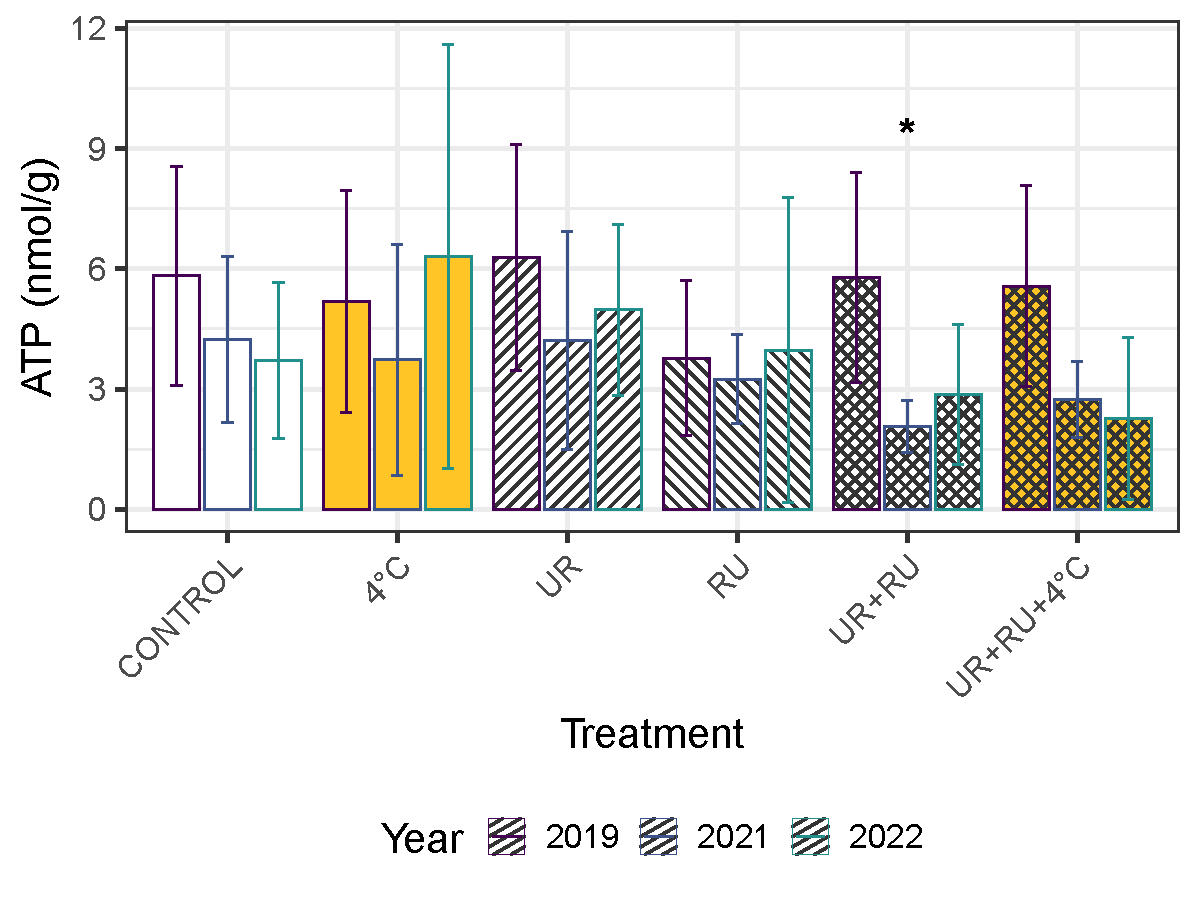
\includegraphics[scale=0.55]{./Figures/ATPSW3Year_barplot_corrected}
    \caption{\textbf{Effects of chemicals on sediment wash ATP in 2019-2022.} There is an antagonistic effect between urban and rural chemical groups in 2019, while a synergistic effect is shown in 2021 and 2022.}
    \label{fig:ATPSW3Year}
\end{figure}

\subsubsection{Microbial respiration}

In 2019-2022, both warming (4°C) and UR+RU significantly and negatively affected microbial respiration (Table \ref{tab:MicroResp_3Year}). In contrast, UR+RU+4°C did not significantly demonstrate an effect on respiration (Figure \ref{fig:MR3Year}).

\begin{figure}[H]
    \centering
    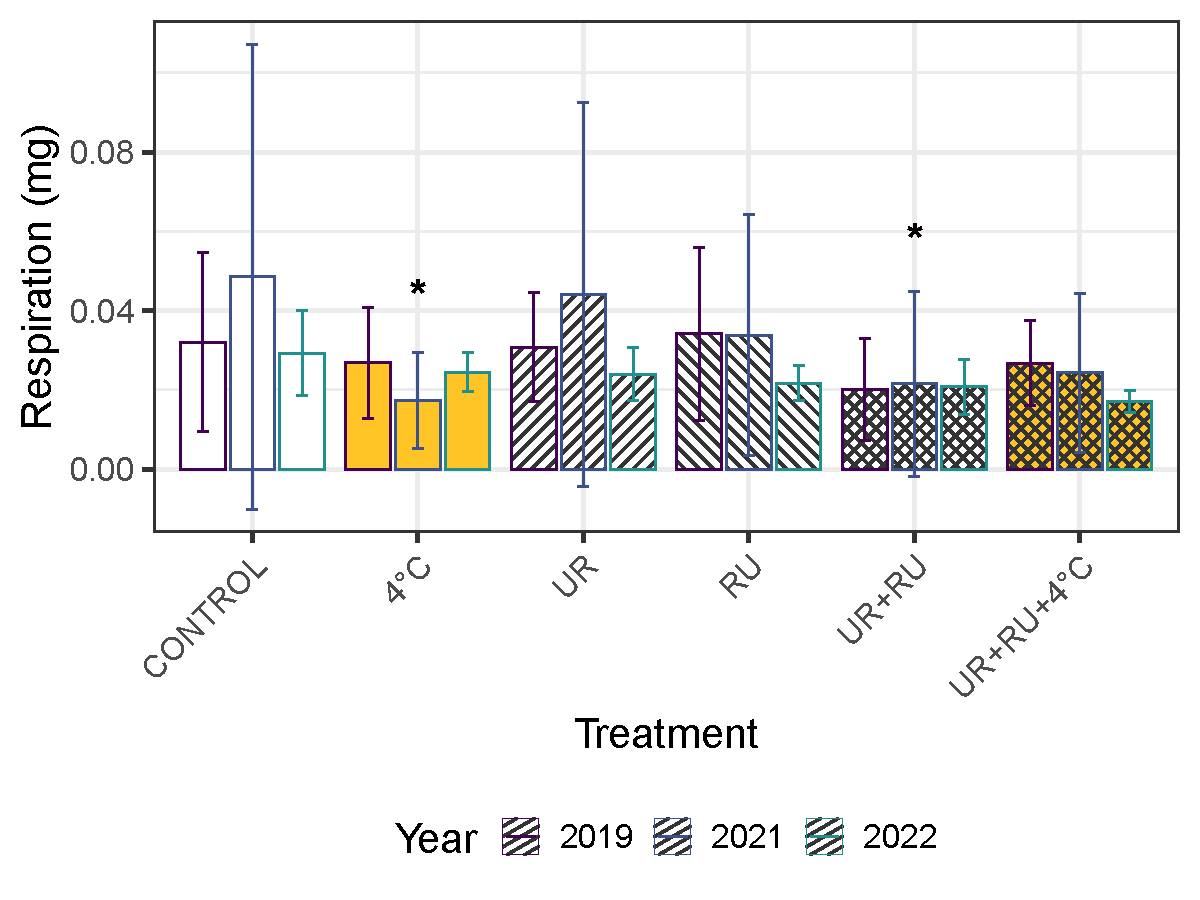
\includegraphics[scale=0.55]{./Figures/MicroResp3Year_bar_corrected}
    \caption{\textbf{Effects of chemicals on microbial respiration in 2019-2022.} Warming (4°C) and UR+RU groups significantly reduced respiration.}
    \label{fig:MR3Year}
\end{figure}

\subsubsection{Decomposition analysis}

A comparison of leaf decomposition three years post-dosing showed that only warming (4°C) significantly affected leaf decomposition in both mesh bags (Table \ref{tab:LD_3Year}). After correcting the temperature, the warming (4°C) treatment only significantly affected leaf decomposition in the fine mesh bags. All showed a positive increase except for the temperature-corrected decomposition of leaves in fine mesh bags.

Leaf decomposition rates were highest in 2022 and lowest in 2021 (Figure \ref{fig:LDTreat}). Consistent with the decomposition of tea bags in 2022, there was an antagonistic effect between RURAL and URBAN chemicals, which was more pronounced under warming (4°C).

\begin{figure}[H]
    \centering
    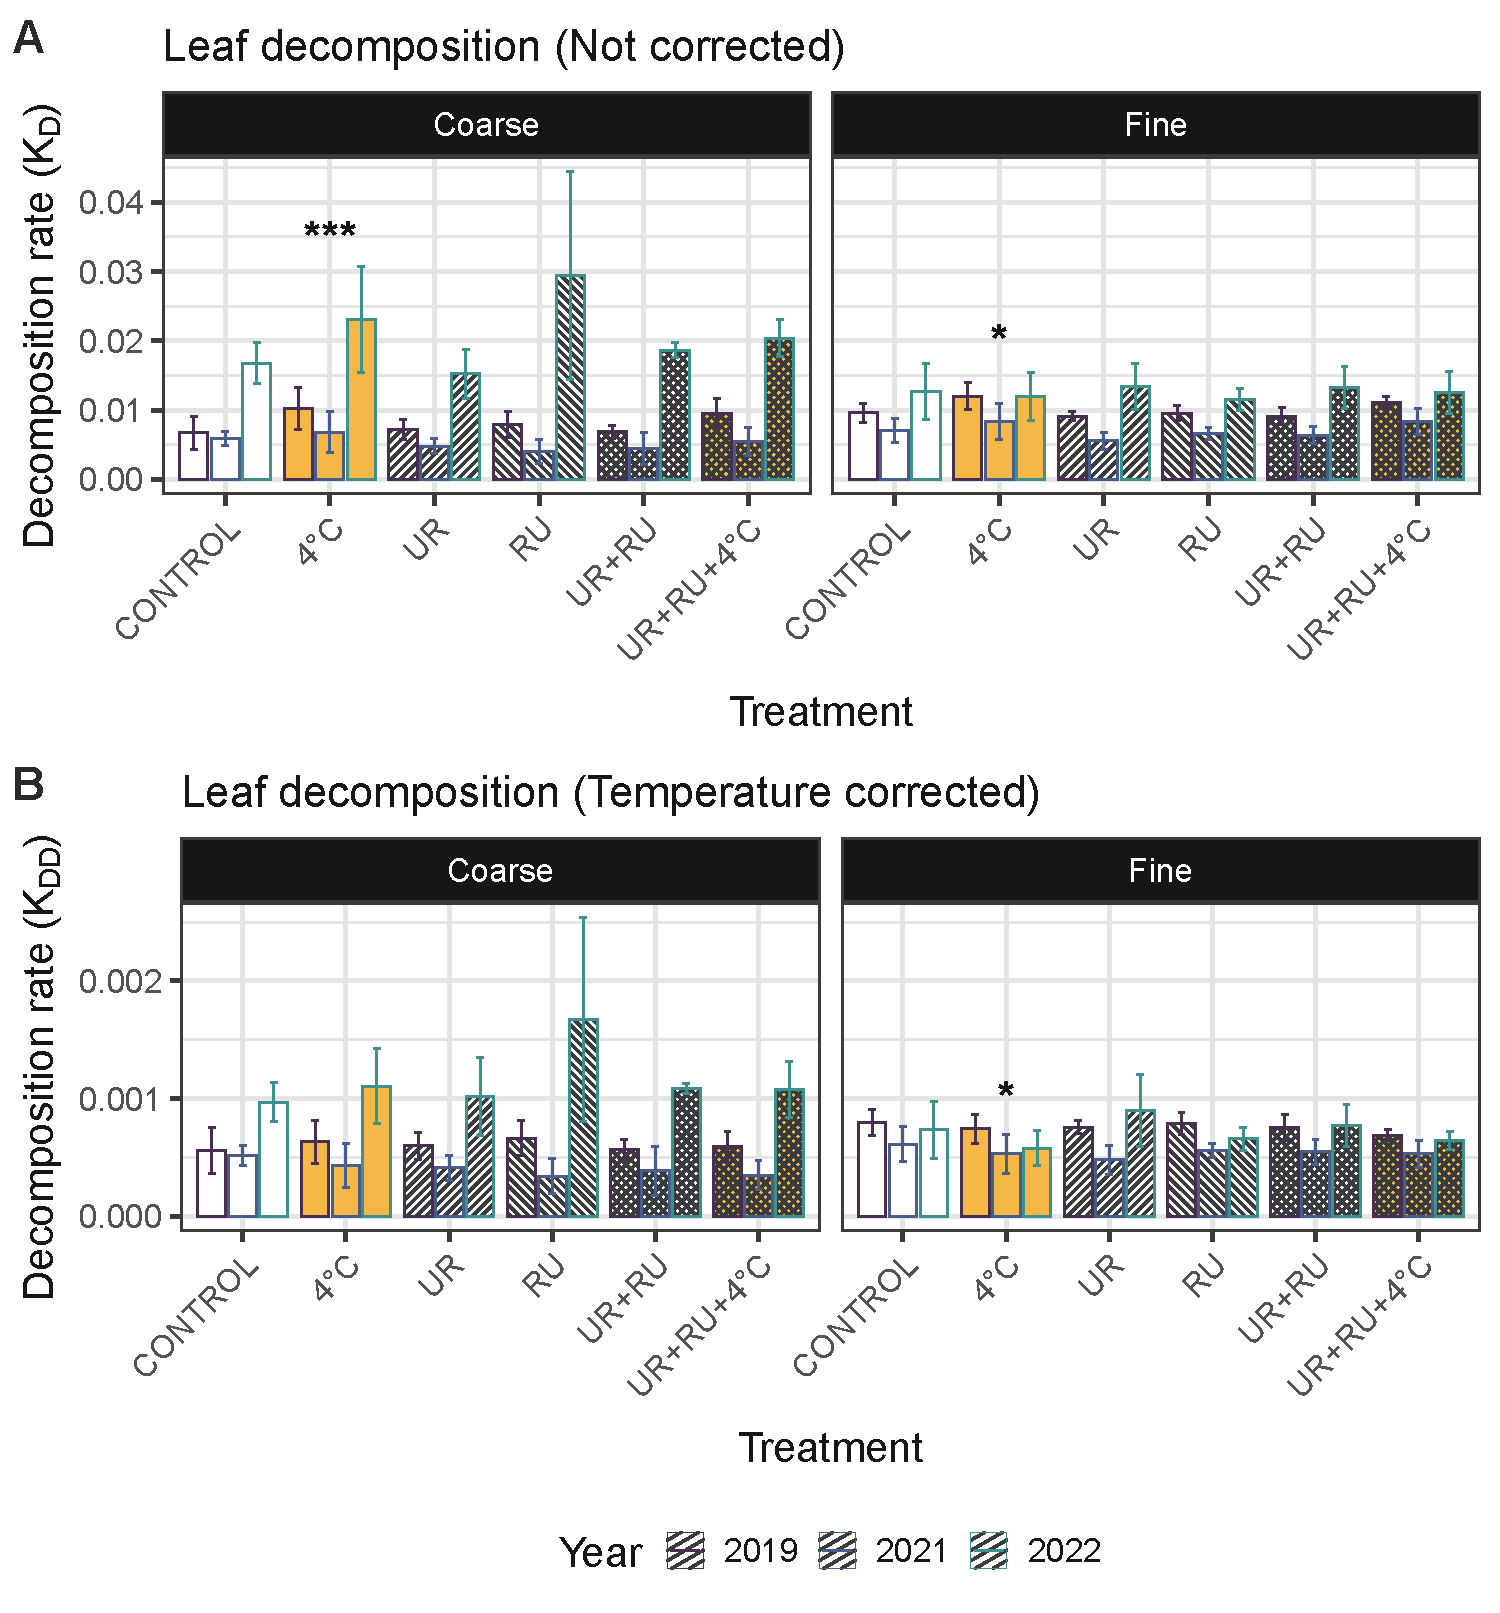
\includegraphics[scale=0.55]{./Figures/LD3Year_bar}
    \caption{\textbf{Effects of chemicals on tea bag decomposition in 2019-2022.} The leaf decomposition rate was the lowest in 2021. Overall the chemical treatments had little effect on the decomposition rate.}
    \label{fig:LDTreat}
\end{figure}


\section{Discussion}

Chemical pollution and global warming are two essential anthropogenic stressors affecting ecosystems \citep{bronmark2002environmental}, and there are potential interactions between them \citep{hooper2013interactions}. This study demonstrates how freshwater microbial community function changes under the stresses of chemicals and warming. The results show that chemicals and warming significantly affect some freshwater microbial functions, depending on the characteristics of the chemical groups and the degree of warming. Of these, chemicals significantly affected ATP production, BOD, microbial respiration, and tea bag decomposition, while gradient warming significantly affected all microbial functions measured except BOD. The existence of antagonistic effects between biocide combinations and warming also confirms that climate can alter the effects of chemicals on organisms.

\subsection{Effects of biocides exposure on the microbial community function in freshwater}

The eight biocides used in this study, representative of those frequently used in urban and rural areas, have been proved to affect the microbial communities in freshwater ecosystems \citep{andreozzi2004antibiotics,barbosa2021resistance,CARABIASMARTINEZ2000471,ernst1991toxicity,keighleyenvironmental,pascault2014high,zhou2020adverse}. In 2022, chemical treatment did not significantly affect ATP production and bacterial respiration, which could support the speculation of this study that the microbial community is redundant in these functions. Metabolic genes have been around since early in Earth's history \citep{david2011rapid}, and over time a vast range of taxa have been able to perform similar metabolic functions \citep{louca2016decoupling}. The hydrological cycle controls freshwater ecosystems, allowing lentic freshwater to possess higher community diversity than lotic freshwater habitats \citep{kuehn2016lentic,roland2010relationships}. The mesocosm facility used in this study reflects the response of lentic freshwater ecosystems to biocides, and the results suggest that the microbial communities in this study are sufficiently diverse to maintain functional stability. BOD as a critical indicator of the oxidation status of a water body reflects the degree of organic pollution in the water body, and biocides significantly affect BOD in this study. UR+RU did not significantly affect BOD in ponds without ammonia treatment (Table \ref{tab:BOD_treat}); however, ammonia-treated ponds significantly reduced this effect. It is possible that under ammonia stress, the microbial community of the pond was altered to increase resistance to the environmental pressure to antibiotic resistance \citep{poole2012stress}, at the same time as the nitrogen source in the water column was increased. For example, there was a significant correlation between the effects of ammonia stress on tetracycline and MLSb resistance genes \citep{zhang2020ammonia}. In ammonia-treated ponds, the decomposition of tea bags was significantly reduced under the pressure of both groups of chemicals (Table \ref{tab:D_2022chem}), which may be related to the presence of free ammonia. The company of free ammonia has a strong inhibitory effect on essential microorganisms responsible for decomposition by breaking down extracellular polymeric substances and causing cell alkalinisation \citep{ferreira2007effect, zhang2018free}, thereby inhibiting bacterial enzyme activity \citep{muller2006ammonium}. The breakdown of extracellular polymers also leads to the easier entry of biocides into the bacteria resulting in cellular inactivation \citep{liu2019roles}.

In 2022, UR+RU significantly affected the BOD of ammonia-treated ponds only (Table \ref{tab:BOD_treat}), with the URBAN and RURAL chemical groups showing a significant synergistic effect, which may be due to the strong synergistic effect of biocides in the presence of ammonia as an environmental stressor. At the same time, their mixing also had a strong synergistic effect on non-target organisms \citep{shahid2019environmental}. However, in other microbial functional assays, the two chemical groups showed non-synergistic results, which may reflect that the increased and decreased toxicity in the mixture counteract each other \citep{deneer2000toxicity}. Most multiple stress effects are antagonistic \citep{folt1999synergism}, and past studies have shown that biocide combinations do not have a more substantial impact on microbial function \citep{hoagland1993freshwater,rossi2018interactive}. Under warming conditions, biocides and temperature showed a significant antagonistic effect. In the ammonia-treated ponds, BOD was significantly higher (Table \ref{tab:BOD_treat}). At the same time, the tea bag decomposition rate was also significantly higher in all ponds (Table \ref{tab:D_2022chem}), suggesting that temperature may have accelerated the volatilisation of ammonia and facilitated the decomposition of some chemicals \citep{op2017negative}. Meanwhile, the increased temperature may have increased the enzymatic activity of microorganisms and promoted the detoxification mechanism of microbial enzymes \citep{chaloupka1985temperature}. Also, the freshwater microbial community in this study was derived from the natural colonisation of the lentic ecosystem around Silwood Park, and the gradual thermal evolution of the higher latitude community with warming may have reduced the impact of biocides \citep{de2013latitudinal}.

Throughout the three years of data, only UR+RU significantly reduced ATP production and microbial respiration, while the rest of the biocide treatments did not significantly affect microbial function (\multiref{tab:ATPSW_3Year}{tab:LD_3Year}). Contrary to the speculation of this study, no ramping effect was shown, which may be related to the fact that the biocides did not have a long-term impact on the microbial community. For example, the half-life of glyphosate at low concentrations was only about five days \citep{perez2007effects}; imidacloprid had no direct effect on bacteria and was safe for freshwater invertebrates at lower concentrations (0.009-0.385 μg/L) \citep{barbosa2021resistance}; amoxicillin and oxytetracycline were not toxic to eukaryotic algae \citep{andreozzi2004antibiotics}, and the concentrations of oxytetracycline in this study were below the resistance of sediment bacteria \citep{samuelsen1992long}; diflufenican was insoluble in the water despite its long half-life and its concentration never exceeded 0.1 μg/L in any case (e.g. in surface water) \citep{CARABIASMARTINEZ2000471}. The resilience of freshwater ecosystems in mesocosm is likely to be more stable, so the microbial community in the sample 32 days after dosing is likely to be after it has recovered. As some biocides affect only the target organisms and a small number of non-target organisms, they may act as a potential source of nutrients for other organisms or interact to create new food webs. Glyphosate is a potential phosphorus source and prevents phytoplankton growth \citep{barbosa2021resistance}, thus reducing the competitive pressure on planktonic bacteria; imidacloprid is toxic to many freshwater invertebrates and also promotes the biomass of planktonic bacteria; tebuconazole can be used as a carbon source by freshwater microbes \citep{pascault2014high}. The combined use of biocides may result in some biocides' delayed or offsetting effects on the microbial community.

\subsection{Effects of warming on the microbial community function in freshwater}

The metabolic theory of ecology suggests that temperature is a fundamental driver of biological metabolic rates \citep{brown2004toward}. With global warming, climate change is causing continued changes in many ecosystem functions over the next hundred years \citep{smith2018predicted}. The diversity and composition of functional genes of microorganisms have a rapid response to temperature changes \citep{barria2013bacterial,wu2017alpine,xue2016tundra}. Gradient warming has a highly significant effect on tea bag decomposition. Linear analysis indicates that the decomposition rate increases with increasing temperature while decreasing after temperature correction (Figure \ref{fig:Tea2022Regression}). Previous studies have shown that warming changes the composition of fungal communities and thus accelerates the decomposition of apoplastic material \citep{dang2009temperature}. As temperature increases, the metabolic rate of bacteria increases, a small proportion of bacteria with high uptake and low respiration rates adapt to higher temperatures, and the resource utilisation capacity of species increases with increasing temperature \citep{smith2019community}. However, tea bag decomposition rates were not significantly related to warming in the ammonia-treated ponds, while decomposition rates decreased more with temperature after correction for temperature. The purpose of temperature correction is to remove the effect of temperature and retain only the effect of other stressors (e.g., climate change, nutrient concentration, light availability, etc.). The results of this study indicate that other stressors significantly affect tea bag decomposition as temperature increases and that this effect is exacerbated by ammonia stress.

Microbial functions such as ATP production, respiration, and BOD did not show a linear relationship with gradient warming (\multiref{fig:ATP2022Regression}{fig:BOD2022Regression}). On the one hand, this may be because microbial functions other than decomposition were assayed under laboratory conditions at the same temperature. These methods may only consider changes in microbial biomass and composition rather than the effect of temperature itself. On the other hand, this may reaffirm the redundancy of microbial community functions. Microbial communities are resistant and resilient at broad but not fine-grained taxonomic levels, with disturbed community composition changing and some taxa of older communities being replaced by phylogenetically close taxa \citep{allison2008resistance}. Warming can weaken or disrupt nutrient interactions within the food web \citep{winder2004climate}, which can be more pronounced in the absence of reliable inputs of nutrients. As the mesocosm facilities used in this study have fewer channels for the exchange of substances with the outside world may lead to nutrient deprivation, and this may make the effect of temperature on the microbial function less obvious \citep{mulholland2010nutrient}. Also, upon exposure to warming, bacteria can alter gene expression machinery to alter cellular resource allocation \citep{de2017resource}, including lower secondary structure genes being translated to coordinate with temperature changes \citep{bartholomaus2016bacteria}. Energy reallocation reduces translation resources for undegraded and newly synthesised mRNAs, which may also be why some microbial functions measured were not significantly associated with warming.

\subsection{Caveats and future directions}

Some of the microbial functioning assays in this study did not reveal effects of biocides and warming on freshwater microbial communities. Therefore, traditional methods of functional assays solely may not fully reveal the effects of stressors on microbial communities. Further work on measuring changes in microbial community function under chemical and warming stresses based on this study could include:

1)	Quantitative PCR (qPCR), mass sequencing of genes, and bioinformatics analysis. Traditional functional assays do not work well due to the possible functional redundancy of the microbial community. After treatment with biocides, the microbial community composition may have changed, but the high diversity is sufficient to maintain functional stability. In the future, qPCR amplification and sequencing could be used to measure better the abundance of microbial functional and taxonomic marker genes, such as 16S rRNA gene abundance as a proxy for total bacterial abundance; ammonia monooxygenase (amoA) abundance from ammonia-oxidising bacteria involved in the N cycle to measure ammonia effect; the cbhl gene is used to measure microbial catabolism, etc.

2)	Standardisation from sampling to experiments. The methods used for sampling and experiments are not completely uniform from one year to the next, leading to data discrepancies. For example, from 2021 onwards, the dilution of the samples used for ATP assay has been modified. At the same time, the data cannot be standardised since part of the considerations for functional assays may have been overlooked, such as the weight and size of Wettex. In the future, the conclusions of this study could be used to supplement and revise the sampling and experimental protocol, ensuring uniformity of work each time.

3)	Increase sampling for acute exposure to biocides. On the one hand, the potentially high resilience stability of freshwater ecosystems in the mesocosm, the short half-lives of some biocides, and interactions result in a poor demonstration of the effects of acute chemical exposure on microbial communities 32 days after dosing. On the other hand, the duration of exposure had a highly significant effect on the microbial community \citep{ding2010effect}. Therefore, sampling at one or two weeks post-dosing could be increased in future studies to investigate changes in microbial function with exposure time.

\section{Conclusion}

This study showed the changes in freshwater microbial community function produced under chemicals and warming stress. Under biocides treatment conditions, ammonia combined with biocides affects more significantly on community function. On the one hand, ammonia stress leads to changes in the microbial community that increase antibiotic resistance. On the other hand, ammonia can have a strong inhibitory effect on the microorganisms responsible for the breakdown of biocides. At the same time, in most cases, chemicals are shown non-synergistic effects on community function among themselves and with warming, which proves that most multiple stress effects are antagonistic. Tea bag decomposition was most affected in the gradient temperature treatment, suggesting that temperature drives the metabolism of the microbial community. Other functional assays were not significantly affected under chemicals and temperature stress, which confirms the existence of redundancy in microbial community function. 2019-2022 do not show a slope effect, which is most likely related to the lack of long-term effects of biocides on microbial communities and the establishment of new food webs in freshwater ecosystems by the combined use of biocides. This study demonstrates the relationship between chemicals and warming stress and freshwater microbial community function and provides improved ideas and new insights for continued research in the future.

\section*{Code Availability}
\addcontentsline{toc}{section}{Code Availability}

The R code for plots and analysis in this study is availible at my github (\href{https://github.com/ChuxuanJi/EECSummerProject}{\color{blue}{\underline{EECSummerProject}}}) repository.

\section*{Acknowledgement}
\addcontentsline{toc}{section}{Acknowledgement}

Above all, I am very grateful to Professor Guy Woodward for his support of my many ideas regarding the experiments of this project and for his supervision of me. Secondly, my heartfelt thanks to Dr Emma Ransome, Dr Tom Smith, Dr Tom Clegg, Danica Duan, Olivia Morris, Laura Kahane, Rhys Preston-Allen and others for their help and support during this project. Thirdly, I am very grateful to my family, girlfriends and friends for giving me the strength and unrequited support to overcome various challenges. Fourthly, I would like to thank Dr Samraat Pawar for helping me to improve my data analysis skills in my first Masters project and for always taking care of me. Fifthly, I really appreciate the security guards at Silwood Park for inspiring me every day. Finally, I greatly thank myself for my love of science and hard working. Each late night at Unit C has recorded my progress and I hope to carry this spirit with me as I continue on my path in microbial ecology.

\addcontentsline{toc}{section}{References}
\bibliographystyle{agsm}
\bibliography{thesis}
\clearpage

\begin{document}
\renewcommand{\thefigure}{SI.\arabic{figure}}
\setcounter{figure}{0}

\renewcommand{\thetable}{SI.\arabic{table}}
\setcounter{table}{0}

\section*{Supplementary Information}\label{sec:SI}

\addcontentsline{toc}{section}{Supplementary Information}
\addtocontents{toc}{\setcounter{tocdepth}{-10}}
\renewcommand{\thesubsection}{SI.\arabic{subsection}}
\setcounter{subsection}{0}


\subsection{Overview}

\begin{figure}[H]
    \centering
    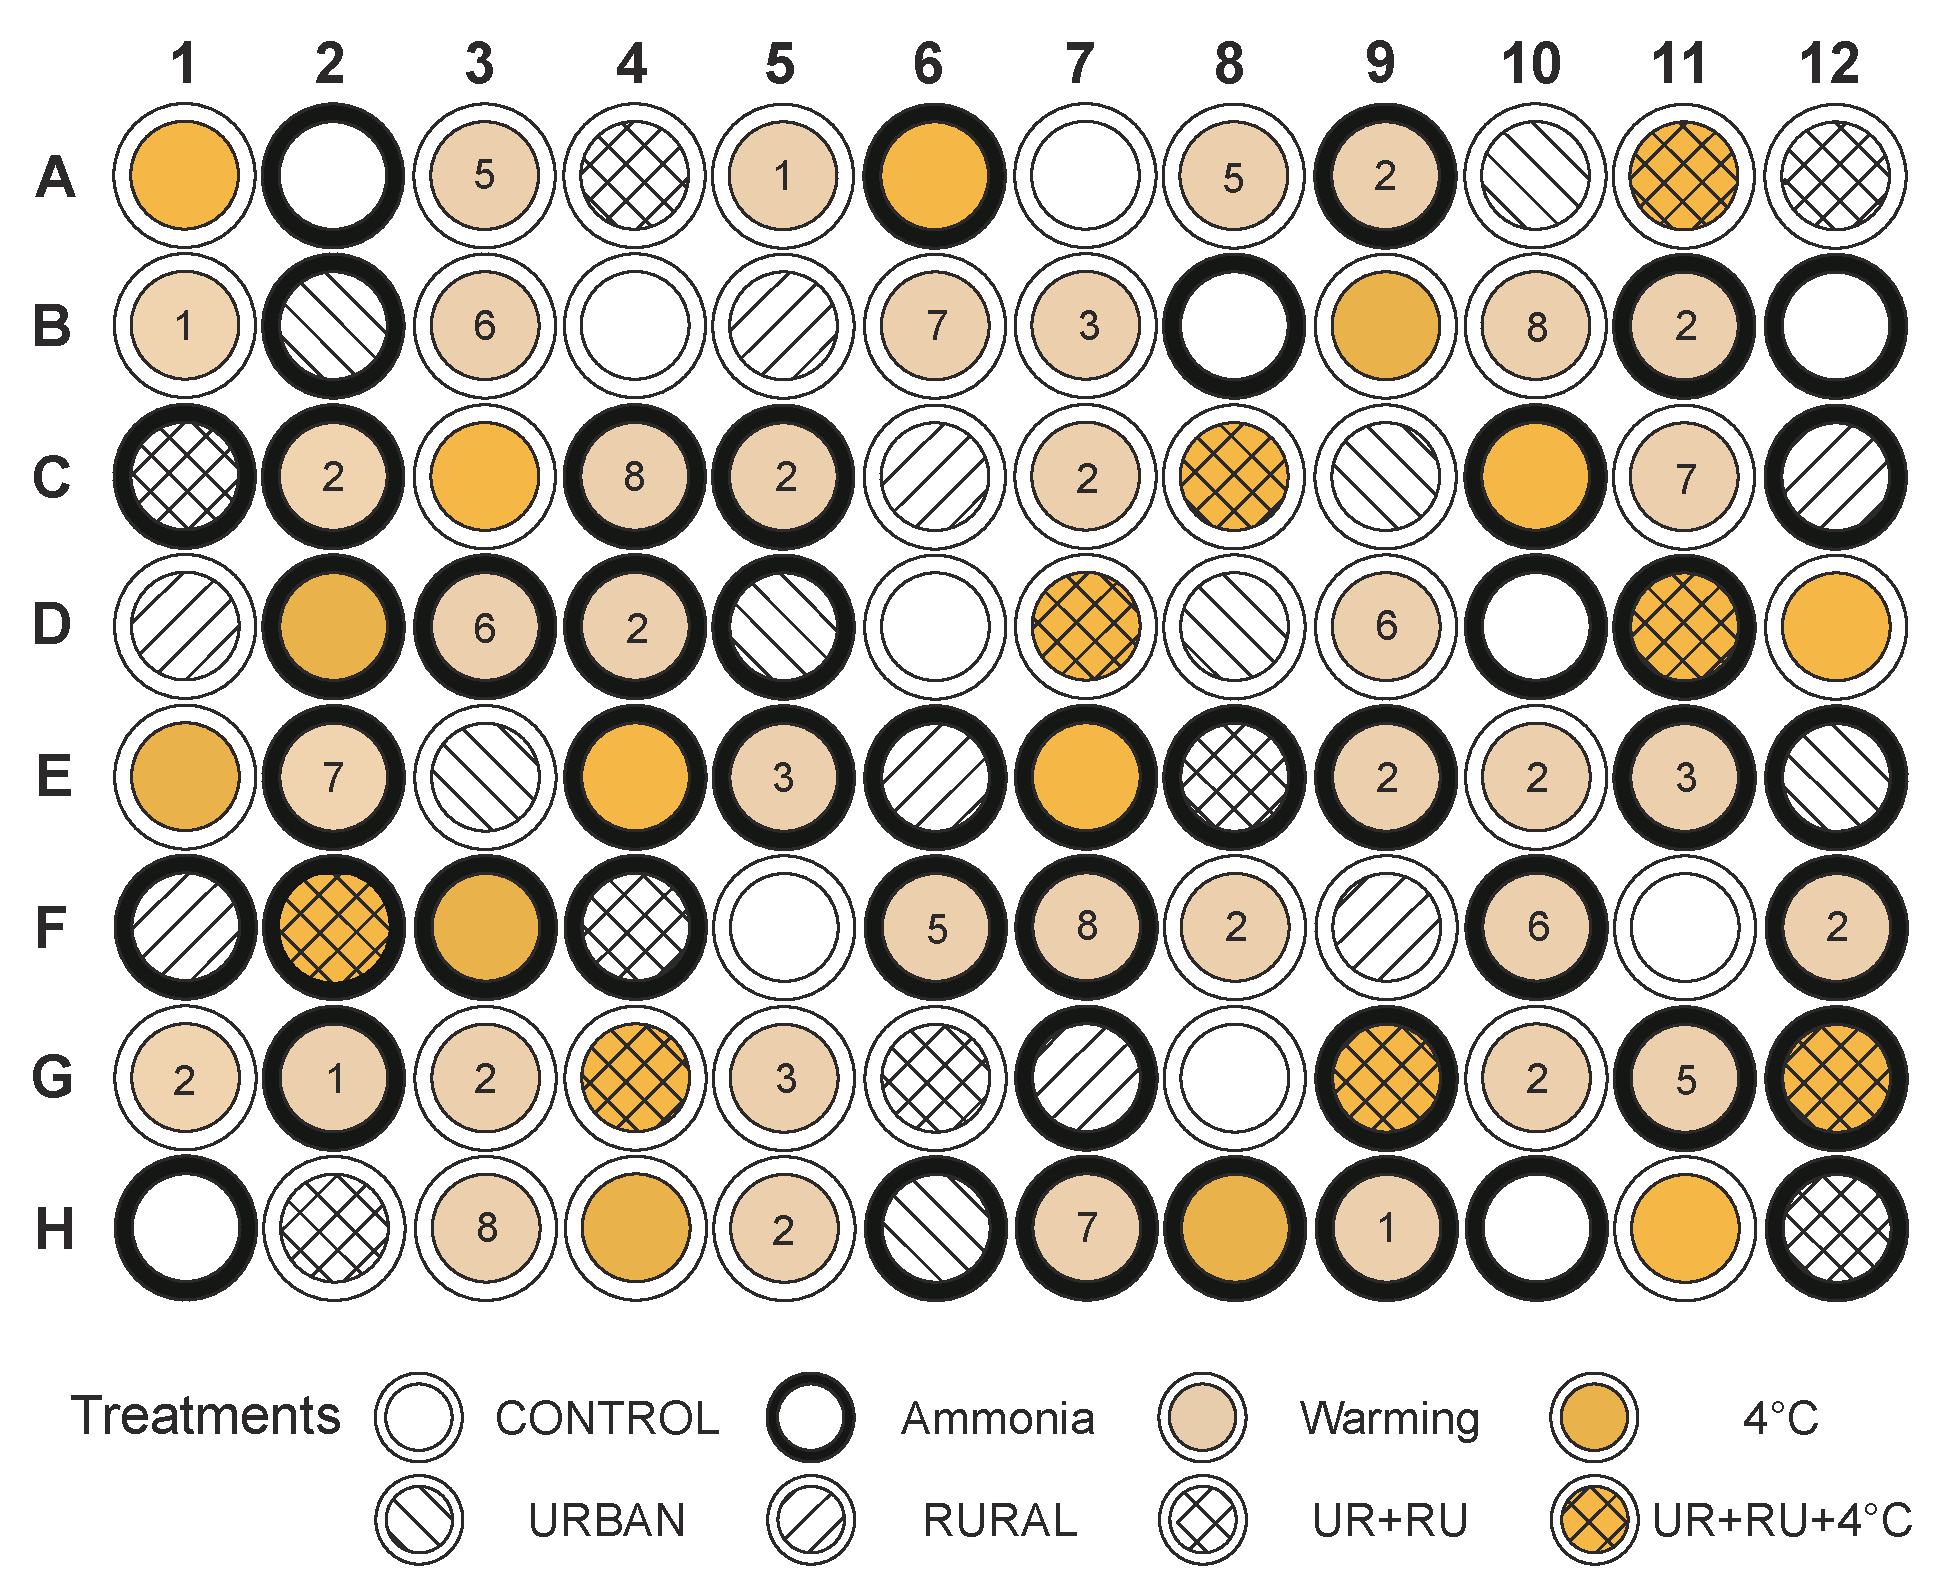
\includegraphics[scale=0.35]{./Figures/Mesocosm}
    \caption{\textbf{Treatment layout of the 96 mesocosms arranged by 8 rows of 12 individual mesocosms.} There are 12 ponds for undisturbed ambient conditions (CONTROL), 8 ponds for the URBAN, RURAL, UR+RU and UR+RU+4°C treatments respectively, and 14 ponds with a 4°C warming. Half of the mesocosms are treated with ammonia (n = 48).}
    \label{fig:Mesocosm}
\end{figure}

\begin{table}[H]
    \caption{\bf The distribution of different treatments.}
    \centering
    \begin{tabular}{ |m{6.6cm}<{\centering}|m{3.5cm}<{\centering}|m{3.5cm}<{\centering}| } 
    \hline
     Treatment & Without Ammonia & Ammonia \\
     \hline
     Control (n=12) & 6 & 6 \\ 
     +1°C (n=4) & 2 & 2 \\
     +2°C (n=14) & 7 & 7 \\
     +3°C (n=4) & 2 & 2 \\
     +4°C (n=14) & 7 & 7 \\
     +5°C (n=4) & 2 & 2 \\
     +6°C (n=4) & 2 & 2 \\
     +7°C (n=4) & 2 & 2 \\
     +8°C (n=4) & 2 & 2 \\
     Urban chemicals (n=8) & 4 & 4 \\
     Rural chemicals (n=8) & 4 & 4 \\
     Urban and rural chemicals (n=8) & 4 & 4 \\
     Urban and rural chemicals, +4°C (n=8) & 4 & 4 \\
    \hline
    \end{tabular}    
    \label{tab:Treatment}
\end{table}

\subsection{Temperature}\label{section:temp}

\begin{figure}[H]
    \centering
    \includegraphics[scale=0.85]{./Figures/Temperature/Mean_month_temp_chem}
    \caption{\textbf{Average monthly temperature of chemical treatment ponds for 2019-2022.} Deep A and B are the different locations of the temperature detectors in the pond.}
    \label{fig:mean_m_temp_chem}
\end{figure}

\begin{figure}[H]
    \centering
    \includegraphics[scale=0.84]{./Figures/Temperature/Mean_month_temp}
    \caption{\textbf{Average monthly temperature of warming treatment ponds for 2019-2022.} Deep A and B are the different locations of the temperature detectors in the pond.}
    \label{fig:mean_m_temp}
\end{figure}

\begin{figure}[H]
    \centering
    \includegraphics[scale=0.78]{./Figures/Temperature/Daily_temp_AB}
    \caption{\textbf{Average daily temperature of the warming treatment ponds for 2019-2022.} Deep A and B are the different locations of the temperature detectors in the pond.}
    \label{fig:d_tempAB}
\end{figure}

\subsection{ATP assays}\label{section:ATPsup}

\begin{figure}[H]
    \centering
    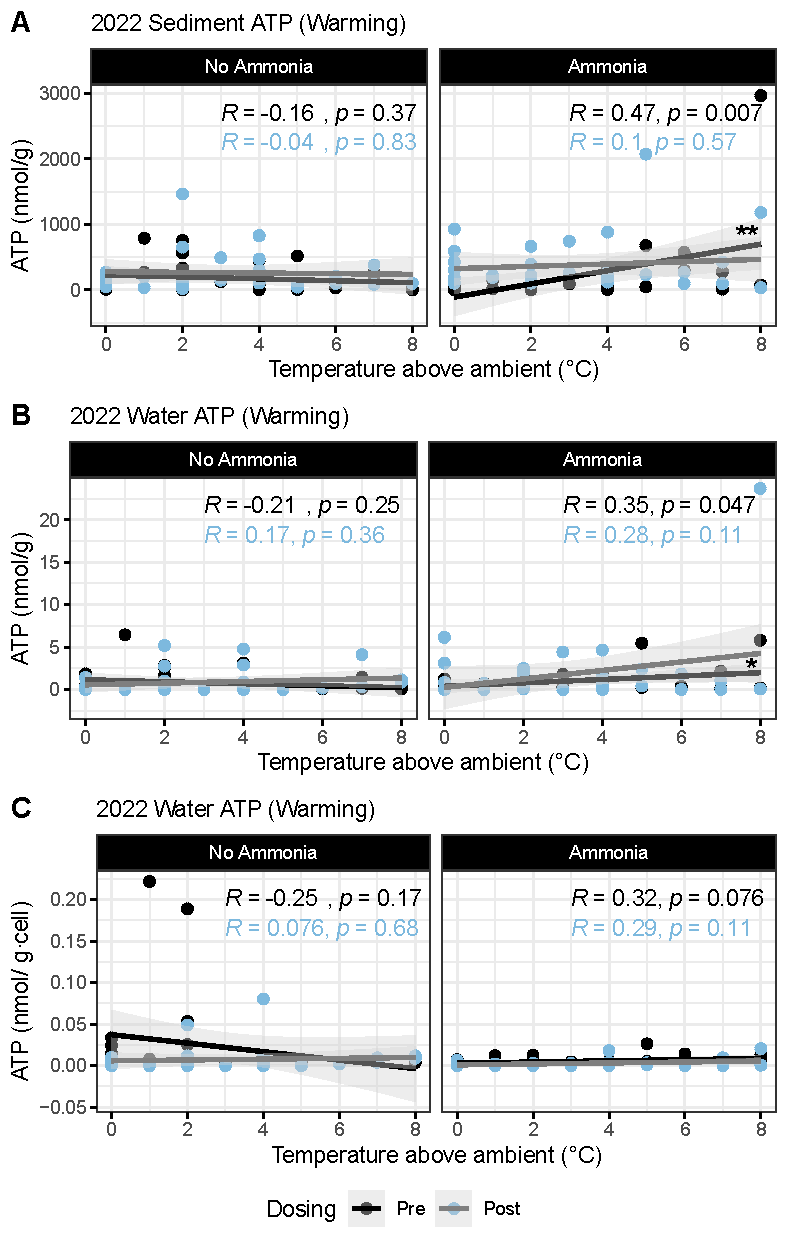
\includegraphics[scale=1]{./Figures/Regression_ATP}
    \caption{\textbf{Trends in ATP production with warming in 2022.} Before dosing, ATP production in sediment and water samples from ammonia-treated ponds increased significantly with warming. After dosing, the gradient warming did not affect ATP production significantly.}
    \label{fig:ATP2022Regression}
\end{figure}

\subsubsection{ATP production from sediment wash samples}

\begin{table}[H]
    \caption{{\bf The performance of LMM (p-values) in determining the effect of different chemical treatments on sediment wash ATP.} All treatments did not significantly affect ATP production.}
    \centering
    \begin{tabular}{ m{2.5cm}<{\centering}m{1.5cm}<{\centering}m{1.5cm}<{\centering}m{1.5cm}<{\centering}m{1.5cm}<{\centering}m{2.2cm}<{\centering}m{2.2cm}<{\centering}}
    \toprule
    Treatment & 4°C & UR & RU & UR+RU & UR+RU+4°C & Temperature \\
     \midrule
    No Ammonia & 0.904 & 0.662 & 0.848 & 0.482 & 0.873 & 0.647 \\
    Ammonia & 0.585 & 0.190 & 0.302 & 0.465 & 0.340 & 0.709 \\
    \bottomrule
    \end{tabular}    
    \label{tab:ATPSW_treat}
\end{table}

In the warming-treated ponds, only the ammonia-treated 5°C warming significantly affected ATP production (Table \ref{tab:ATPSW_temp}), and in a positive direction.

\begin{table}[H]
    \caption{{\bf The performance of LMM (p-values and effect sizes) in determining the effect of different temperature treatments on 2022 sediment wash ATP.} Where p-values are \textless 0.05, they are shown in bold and the effect size (Cohen's d) is in the corresponding parentheses below. The 5°C warming with ammonia treatment significantly affected ATP production, which is due to the extremely high ATP production in G11 ponds (which is associated with high biomass in G11 ponds).}
    \centering
    \begin{tabular}{ m{2.5cm}<{\centering}m{1.2cm}<{\centering}m{1.2cm}<{\centering}m{1.2cm}<{\centering}m{1.2cm}<{\centering}m{1.2cm}<{\centering}m{1.2cm}<{\centering}m{1.2cm}<{\centering}m{1.2cm}<{\centering}} 
    \toprule
    Treatment & 1°C & 2°C & 3°C & 4°C & 5°C & 6°C & 7°C & 8°C \\
     \midrule
    No Ammonia & 0.692 & 0.077 & 0.761 & 0.904 & 0.636 & 0.877 & 0.996 & 0.544 \\
    \multirow{2}*{Ammonia} & 0.747 & 0.654 & 0.401 & 0.585 & \textbf{\textless 0.001} & 0.519 & 0.711 & 0.963 \\
     &  &  &  &  & (1.21) &  &  &  \\
    \bottomrule
    \end{tabular}    
    \label{tab:ATPSW_temp}
\end{table}

\begin{figure}[H]
    \centering
    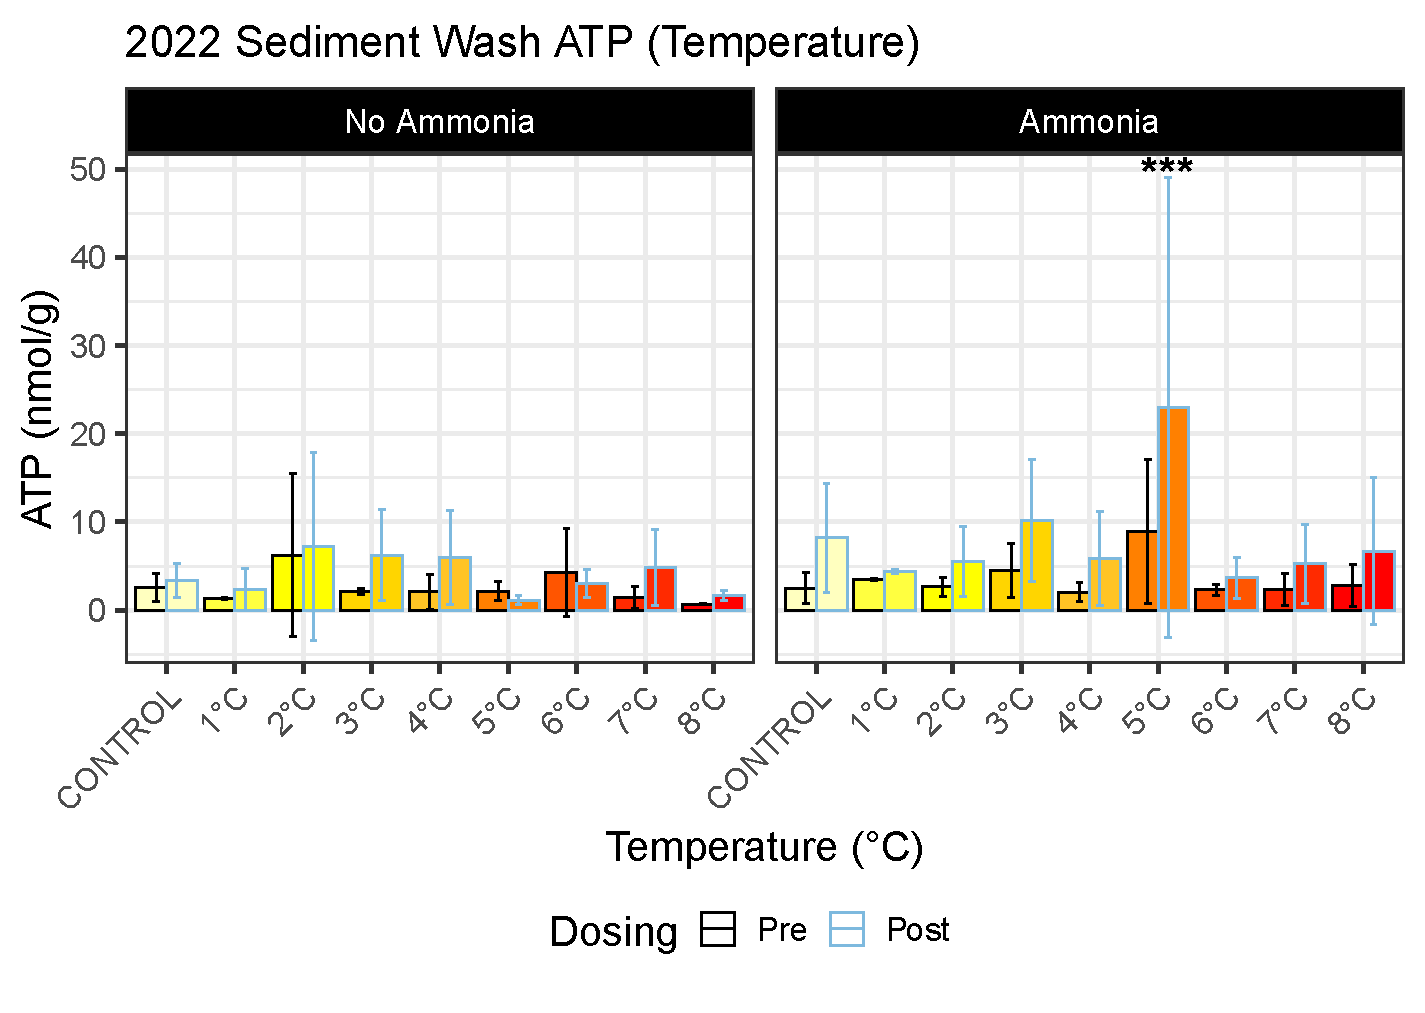
\includegraphics[scale=0.5]{./Figures/ATPSW2022_bar_temp}
    \caption{\textbf{Effects of gradient warming on microbial ATP production in 2022.} Half of the 96 ponds were treated with ammonia. 5°C warming significantly increased ATP production.}
    \label{fig:ATPSW2022_temp}
\end{figure}

\subsubsection{ATP production from sediment samples}

\begin{table}[H]
    \caption{{\bf The performance of LMM (p-values) in determining the effect of different chemical treatments on sediment ATP.} All treatments did not significantly affect ATP production. }
    \centering
    \begin{tabular}{ m{2.5cm}<{\centering}m{1.5cm}<{\centering}m{1.5cm}<{\centering}m{1.5cm}<{\centering}m{1.5cm}<{\centering}m{2.2cm}<{\centering}m{2.2cm}<{\centering}}
    \toprule
    Treatment & 4°C & UR & RU & UR+RU & UR+RU+4°C & Temperature \\
     \midrule
    No Ammonia & 0.517 & 0.627 & 0.419 & 0.216 & 0.700 & 0.390 \\
    Ammonia & 0.595 & 0.990 & 0.684 & 0.703 & 0.720 & 0.115 \\
    \bottomrule
    \end{tabular}    
    \label{tab:ATPS_treat}
\end{table}

\begin{table}[H]
    \caption{{\bf The performance of LMM (p-values and effect sizes) in determining the effect of different temperature treatments on 2022 sediment ATP.} Where p-values are \textless 0.05, they are shown in bold and the effect size (Cohen's d) is in the corresponding parentheses below. Only 8°C warming in ammonia-treated ponds significantly increased ATP production.}
    \centering
    \begin{tabular}{ m{2.5cm}<{\centering}m{1.2cm}<{\centering}m{1.2cm}<{\centering}m{1.2cm}<{\centering}m{1.2cm}<{\centering}m{1.2cm}<{\centering}m{1.2cm}<{\centering}m{1.2cm}<{\centering}m{1.2cm}<{\centering}} 
    \toprule
    Treatment & 1°C & 2°C & 3°C & 4°C & 5°C & 6°C & 7°C & 8°C \\
     \midrule
    No Ammonia & 0.319 & 0.095 & 0.740 & 0.517 & 0.840 & 0.577 & 0.718 & 0.326 \\
    \multirow{2}*{Ammonia} & 0.405 & 0.223 & 0.926 & 0.595 & 0.098 & 0.870 & 0.544 & \textbf{0.005} \\
     &  &  &  &  &  &  &  & (0.95) \\
    \bottomrule
    \end{tabular}    
    \label{tab:ATPS_temp}
\end{table}

\begin{figure}[H]
    \centering
    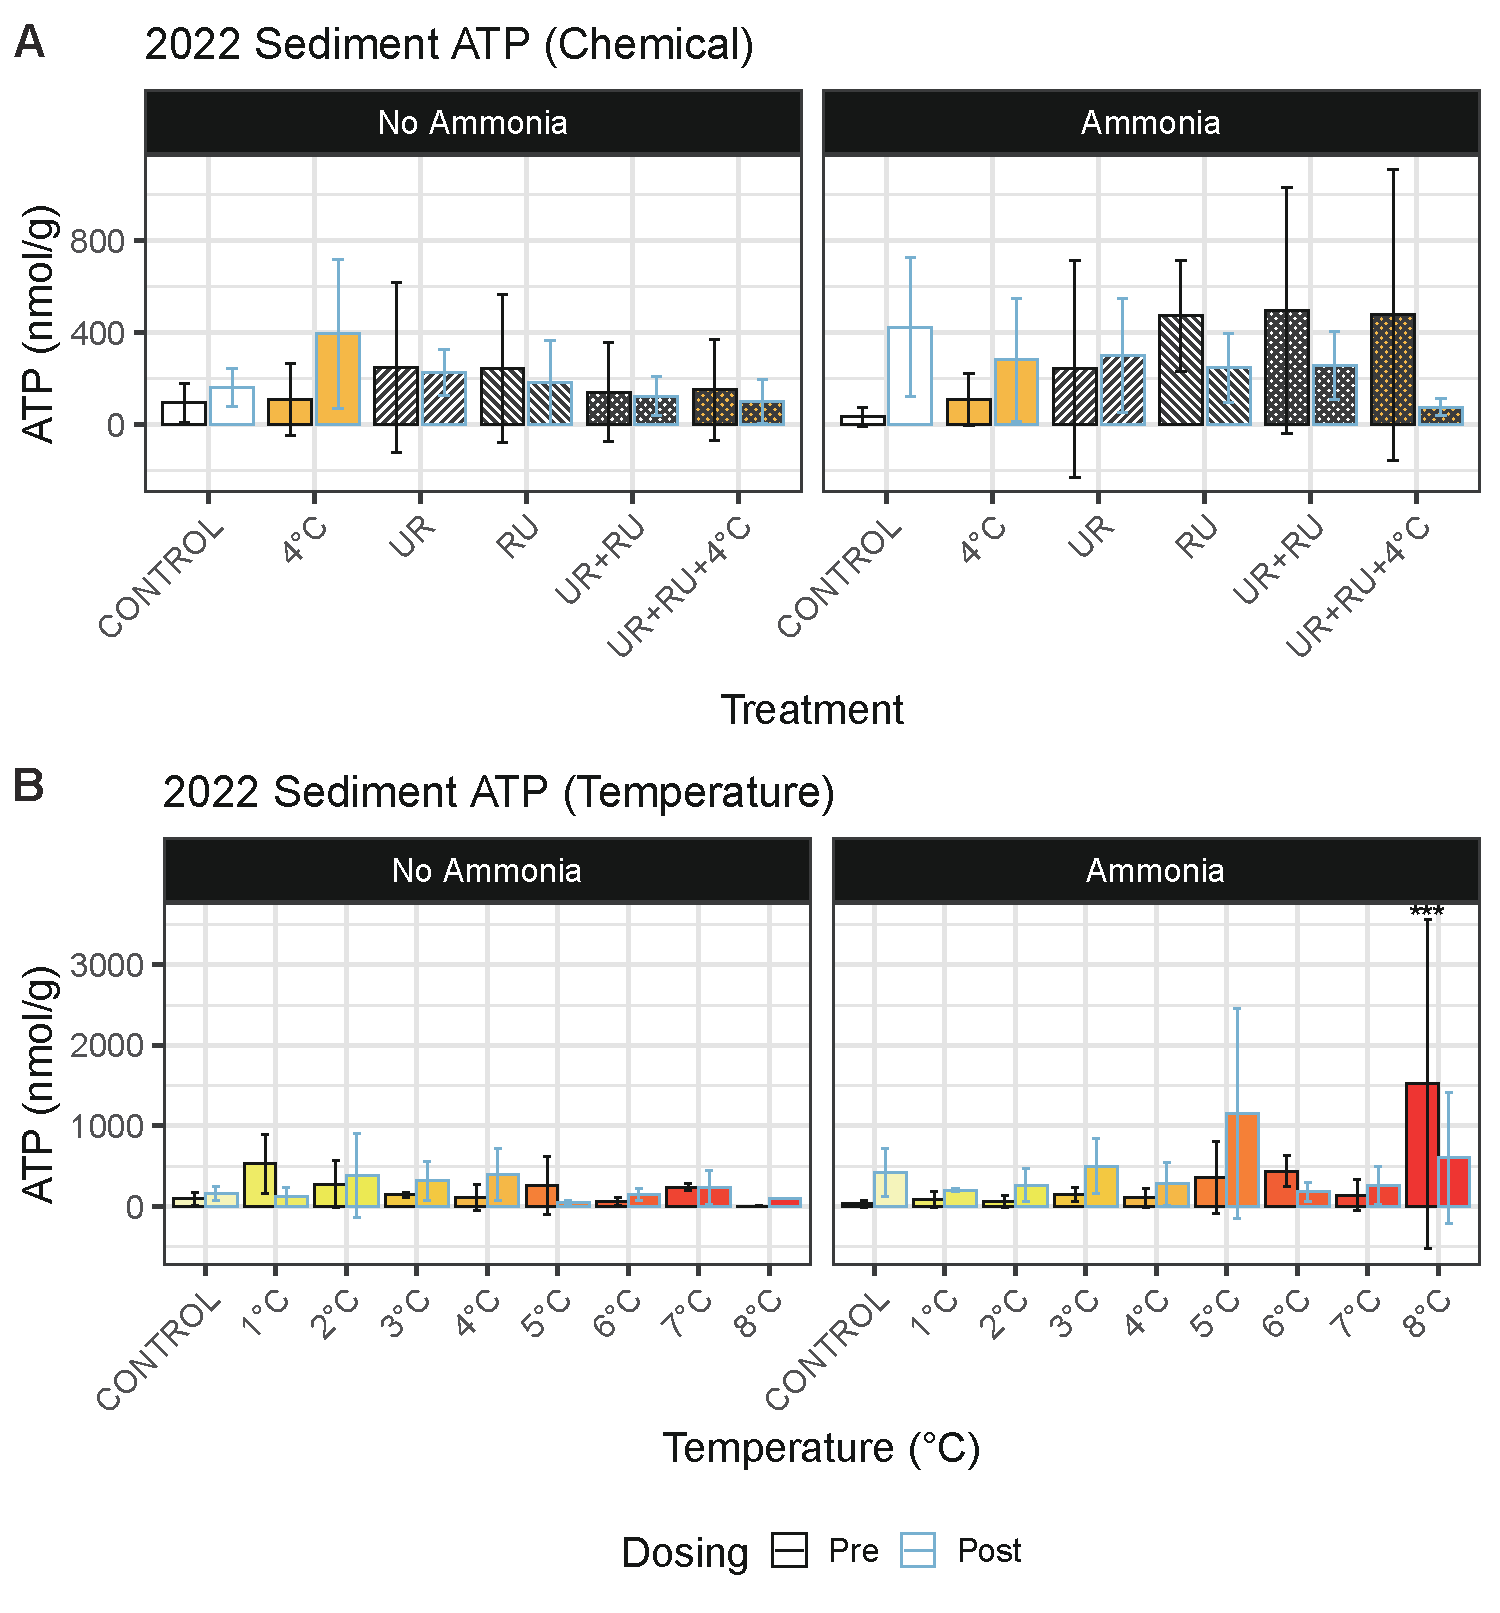
\includegraphics[scale=0.5]{./Figures/ATPS2022_bar}
    \caption{\textbf{Effects of chemical and gradient warming treatment on sediment microbial ATP production in 2022.} Biocides had an opposite effect on ATP production without and with ammonia treatment. The biocide significantly reduced ATP production through a synergistic effect with warming. In the ammonia-treated ponds, both 5 and 8°C warming significantly increased ATP production (which may be related to the abundance of biomass in ponds G11 and F7 respectively).}
    \label{fig:ATPS2022_bar}
\end{figure}

\subsubsection{ATP production from water samples}

\begin{table}[H]
    \caption{{\bf The performance of LMM (p-values and effect sizes) in determining the effect of different chemical treatments on water ATP.} Where p-values are \textless 0.05, they are shown in bold and the effect size (Cohen's d) is in the corresponding parentheses below. Only in the ammonia-treated ponds did gradient warming significantly increase the ATP production of the water samples.}
    \centering
    \begin{tabular}{ m{2.5cm}<{\centering}m{1.5cm}<{\centering}m{1.5cm}<{\centering}m{1.5cm}<{\centering}m{1.5cm}<{\centering}m{2.2cm}<{\centering}m{2.2cm}<{\centering}}
    \toprule
    Treatment & 4°C & UR & RU & UR+RU & UR+RU+4°C & Temperature \\
     \midrule
    No Ammonia & 0.133 & 0.468 & 0.735 & 0.872 & 0.209 & 0.646 \\
    \multirow{2}*{Ammonia} & 0.741 & 0.812 & 0.757 & 0.765 & 0.907 & \textbf{0.039} \\
     &  &  &  &  &  & (0.58) \\
    \bottomrule
    \end{tabular}    
    \label{tab:ATPW_treat}
\end{table}

\begin{table}[H]
    \caption{{\bf The performance of LMM (p-values and effect sizes) in determining the effect of different temperature treatments on 2022 water ATP.} Where p-values are \textless 0.05, they are shown in bold and the effect size (Cohen's d) is in the corresponding parentheses below. Under ammonia treatment, an 8°C warming significantly increased ATP production.}
    \centering
    \begin{tabular}{ m{2.5cm}<{\centering}m{1.2cm}<{\centering}m{1.2cm}<{\centering}m{1.2cm}<{\centering}m{1.2cm}<{\centering}m{1.2cm}<{\centering}m{1.2cm}<{\centering}m{1.2cm}<{\centering}m{1.2cm}<{\centering}} 
    \toprule
    Treatment & 1°C & 2°C & 3°C & 4°C & 5°C & 6°C & 7°C & 8°C \\
     \midrule
    No Ammonia & 0.129 & 0.11 & 0.649 & 0.133 & 0.776 & 0.711 & 0.179 & 0.871 \\
    \multirow{2}*{Ammonia} & 0.710 & 0.994 & 0.670 & 0.742 & 0.437 & 0.986 & 0.919 & \textbf{\textless 0.001} \\
     &  &  &  &  &  &  &  & (1.37) \\
    \bottomrule
    \end{tabular}    
    \label{tab:ATPW_temp}
\end{table}

\begin{figure}[H]
    \centering
    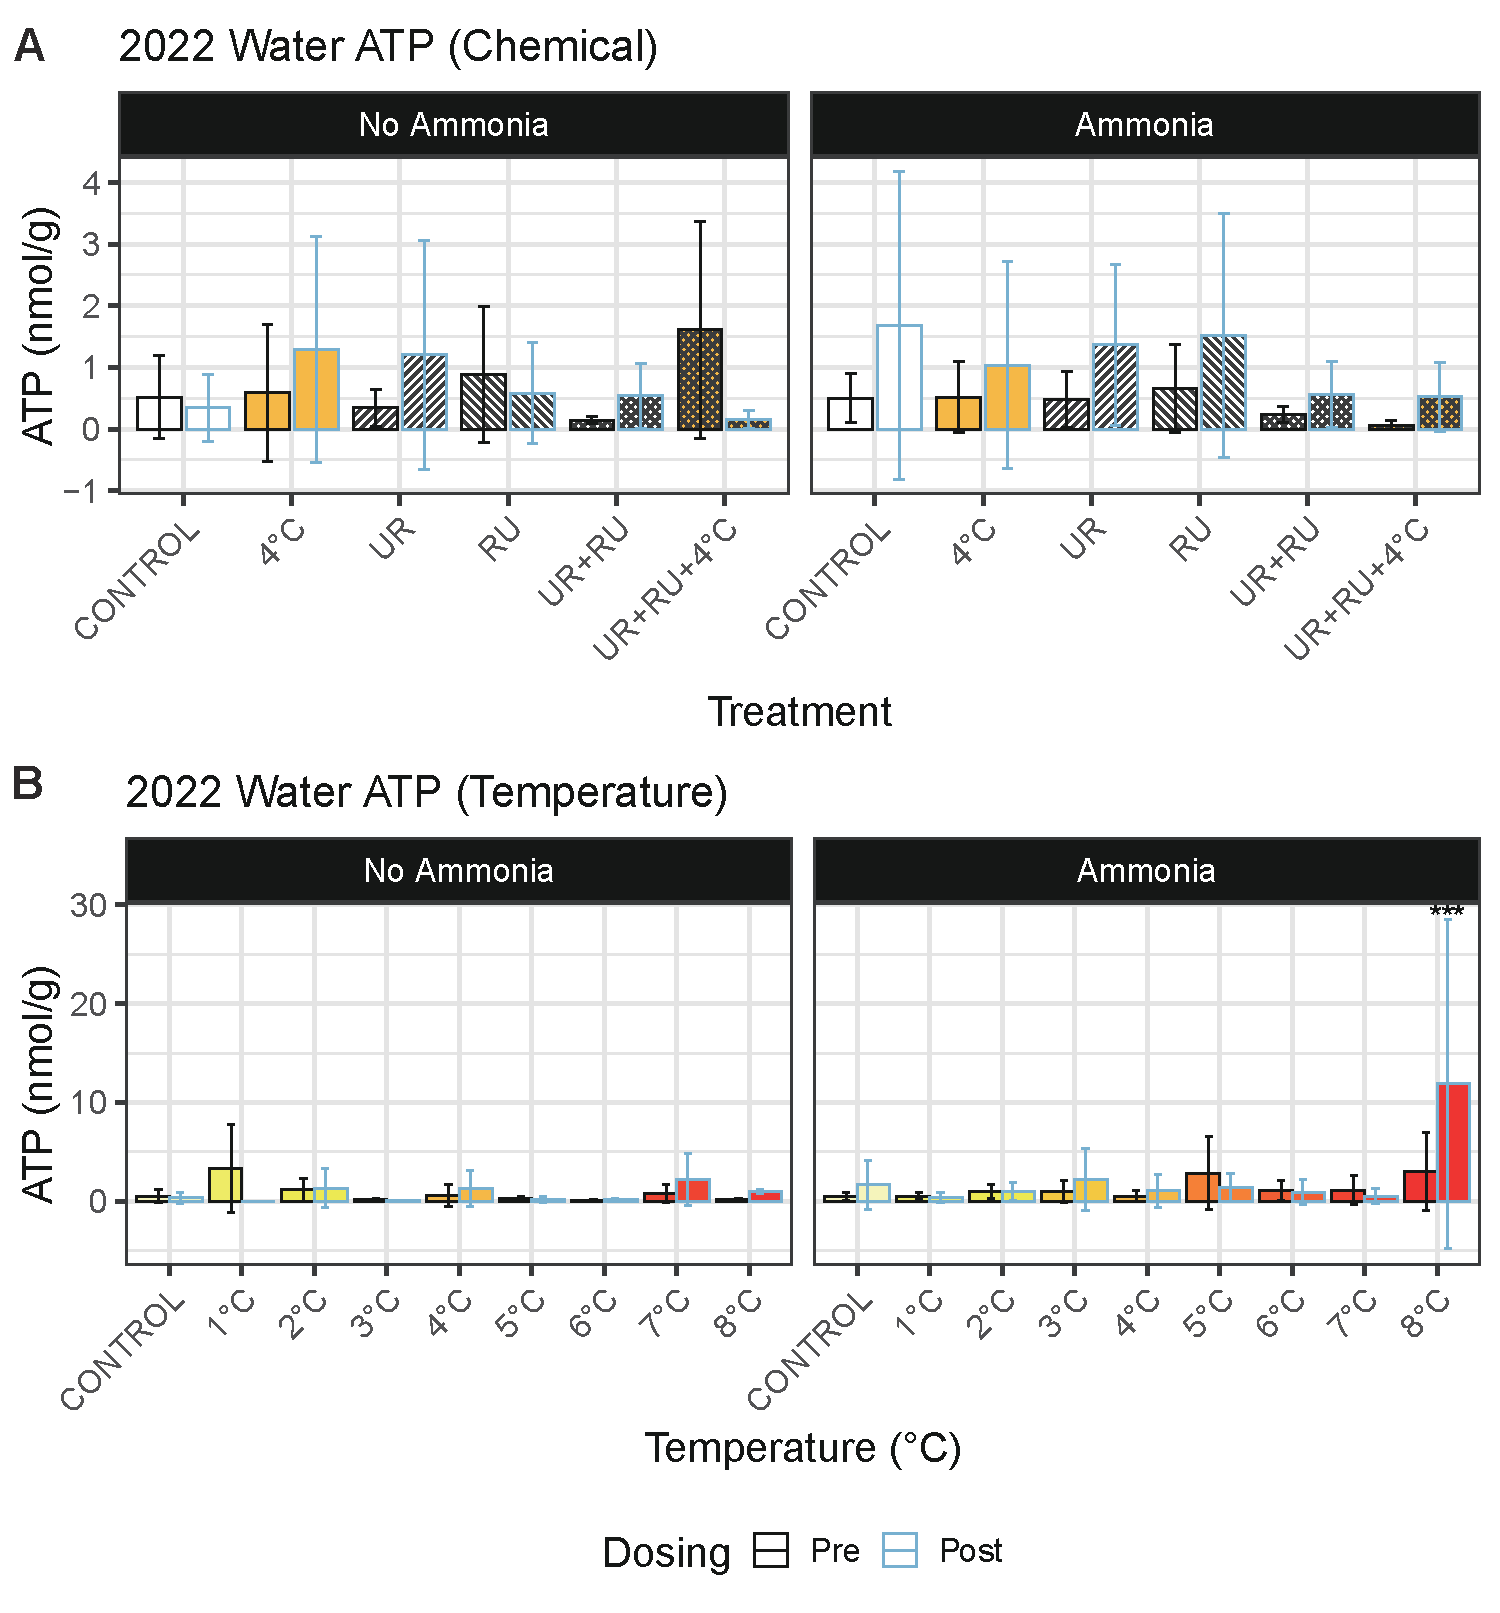
\includegraphics[scale=0.5]{./Figures/ATPW2022_bar}
    \caption{\textbf{Effects of chemical and gradient warming treatment on water microbial ATP production in 2022.} Biocides had an opposite effect on ATP production without and with ammonia treatment. The biocide significantly reduced ATP production through a synergistic effect with warming. In the ammonia-treated ponds, only 8°C warming significantly increased ATP production (which may be also related to the abundance of biomass in F7 pond).}
    \label{fig:ATPW2022_cp}
\end{figure}

\begin{table}[H]
    \caption{{\bf The performance of LMM (p-values and effect sizes) in determining the effect of different chemical treatments on water ATP (per-cell).} All treatments did not significantly affect ATP production.}
    \centering
    \begin{tabular}{ m{2.5cm}<{\centering}m{1.5cm}<{\centering}m{1.5cm}<{\centering}m{1.5cm}<{\centering}m{1.5cm}<{\centering}m{2.2cm}<{\centering}m{2.2cm}<{\centering}}
    \toprule
    Treatment & 4°C & UR & RU & UR+RU & UR+RU+4°C & Temperature \\
     \midrule
    No Ammonia & 0.208 & 0.989 & 0.803 & 0.989 & 0.482 & 0.702 \\
    Ammonia & 0.258 & 0.125 & 0.127 & 0.394 & 0.611 & 0.854 \\
    \bottomrule
    \end{tabular}    
    \label{tab:ATPpc_treat}
\end{table}

\begin{table}[H]
    \caption{{\bf The performance of LMM (p-values and effect sizes) in determining the effect of different temperature treatments on 2022 water ATP (per-cell).} Where p-values are \textless 0.05, they are shown in bold and the effect size (Cohen's d) is in the corresponding parentheses below. Only 1°C warming significantly increased ATP production.}
    \centering
    \begin{tabular}{ m{2.5cm}<{\centering}m{1.2cm}<{\centering}m{1.2cm}<{\centering}m{1.2cm}<{\centering}m{1.2cm}<{\centering}m{1.2cm}<{\centering}m{1.2cm}<{\centering}m{1.2cm}<{\centering}m{1.2cm}<{\centering}} 
    \toprule
    Treatment & 1°C & 2°C & 3°C & 4°C & 5°C & 6°C & 7°C & 8°C \\
     \midrule
    \multirow{2}*{No Ammonia} & \textbf{0.029} & 0.198 & 0.732 & 0.208 & 0.791 & 0.795 & 0.939 & 0.968 \\
     & (0.49) &  &  &  &  &  &  &  \\
    Ammonia & 0.617 & 0.207 & 0.396 & 0.258 & 0.633 & 0.618 & 0.774 & 0.418 \\
    \bottomrule
    \end{tabular}    
    \label{tab:ATPpc_temp}
\end{table}

\begin{figure}[H]
    \centering
    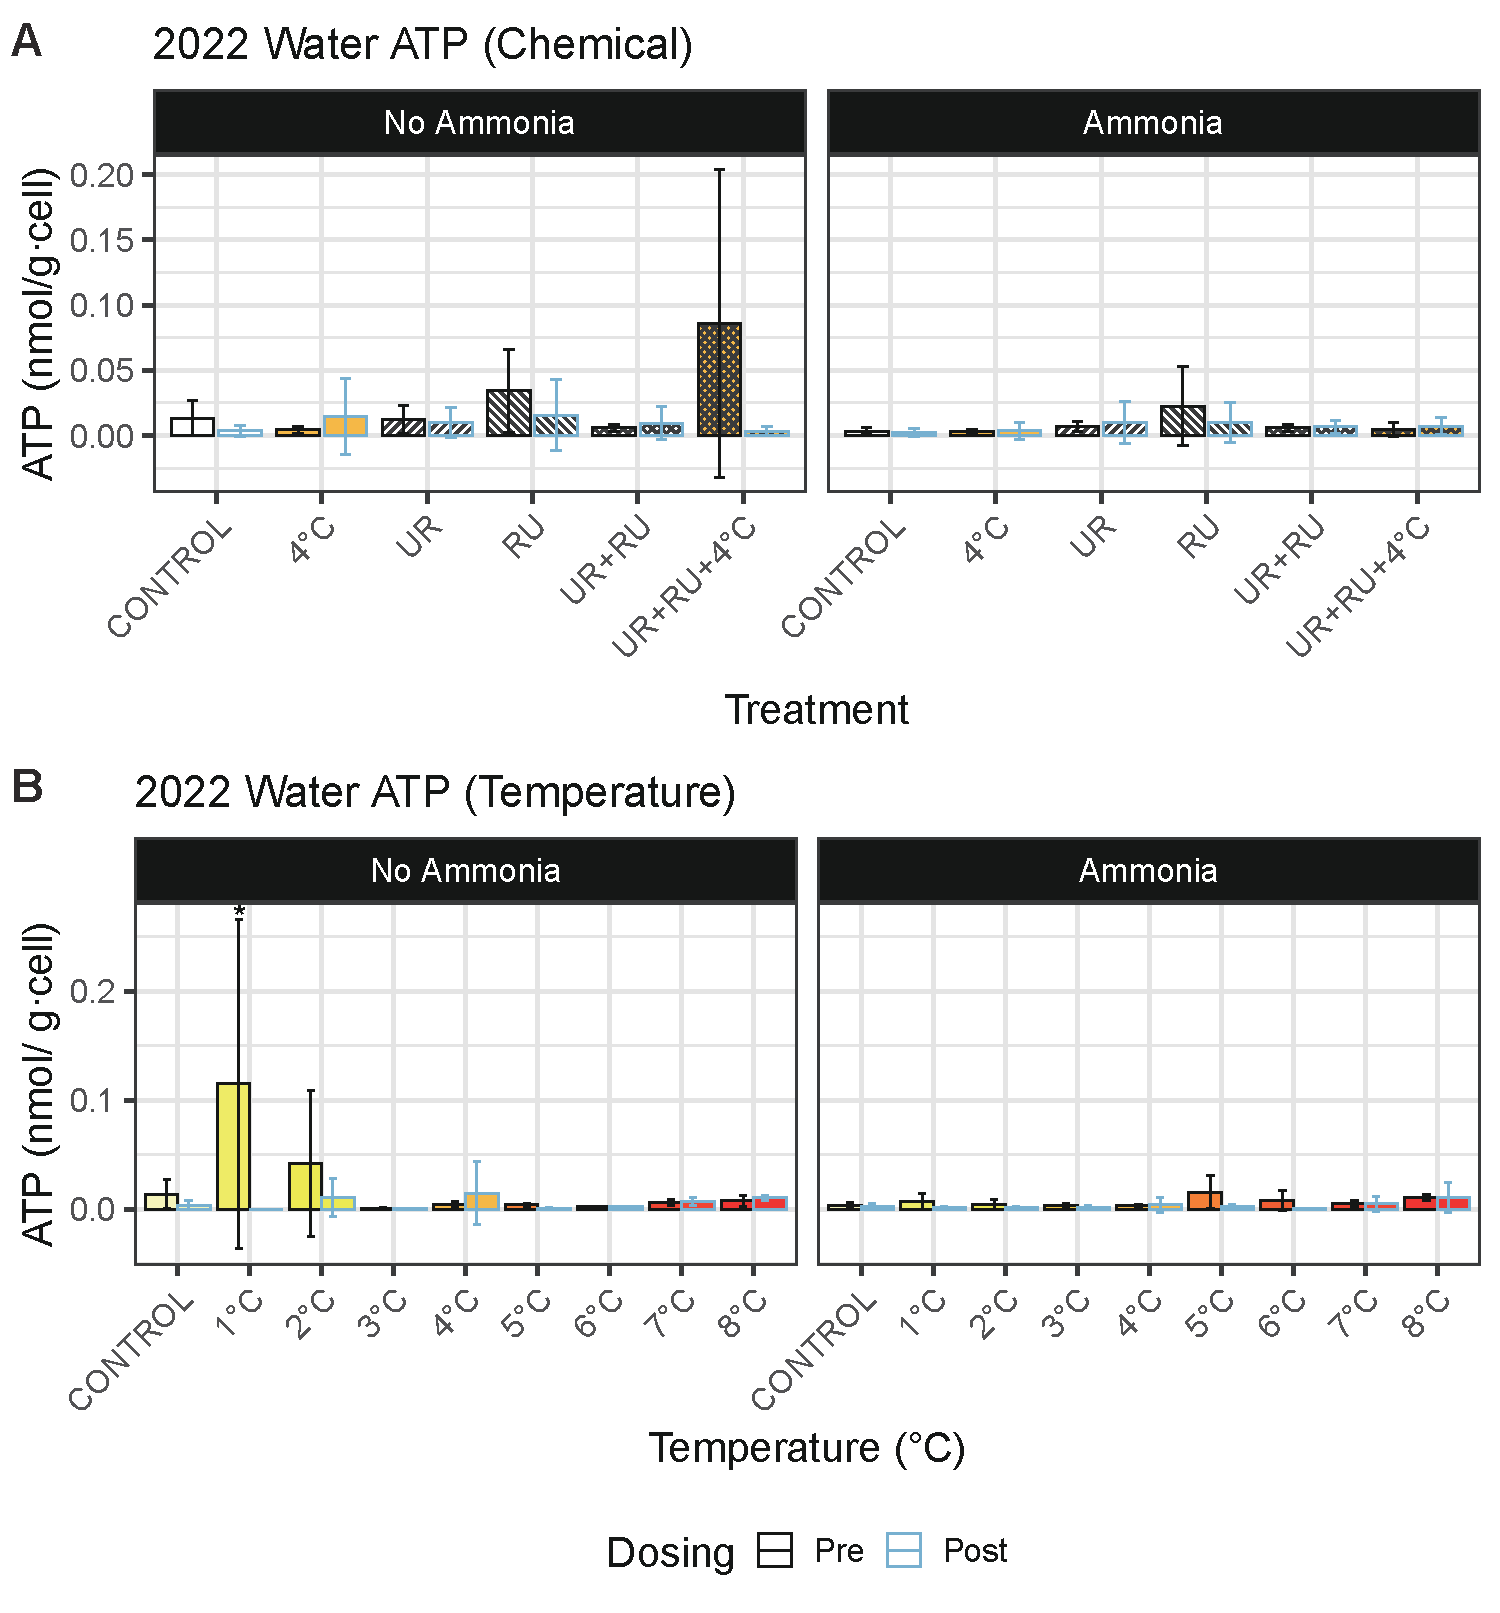
\includegraphics[scale=0.5]{./Figures/ATPWpc2022_bar}
    \caption{\textbf{Effects of chemical and gradient warming treatment on cell microbial ATP production of water samples in 2022.} Only 1°C warming significantly increased ATP production (which may be related to the B1 pond).}
    \label{fig:ATPpc2022_cp}
\end{figure}

\subsection{MicroResp}\label{section:MRS}

\begin{table}[H]
    \caption{{\bf The performance of LMM (p-values and effect sizes) in determining the effect of different chemical treatments on sediment wash MicroResp.} All treatments did not significantly affect microbial respiration.}
    \centering
    \begin{tabular}{ m{2.5cm}<{\centering}m{1.5cm}<{\centering}m{1.5cm}<{\centering}m{1.5cm}<{\centering}m{1.5cm}<{\centering}m{2.2cm}<{\centering}m{2.2cm}<{\centering}}
    \toprule
    Treatment & 4°C & UR & RU & UR+RU & UR+RU+4°C & Temperature \\
     \midrule
    No Ammonia & 0.690 & 0.564 & 0.275 & 0.136 & 0.537 & 0.412 \\
    Ammonia & 0.956 & 0.476 & 0.718 & 0.921 & 0.191 & 0.544 \\
    \bottomrule
    \end{tabular}    
    \label{tab:MR_treat}
\end{table}

\begin{table}[H]
    \caption{{\bf The performance of LMM (p-values and effect sizes) in determining the effect of different temperature treatments on 2022 sediment wash MicroResp.} All warming treatments did not significantly affect microbial respiration.}
    \centering
    \begin{tabular}{ m{2.5cm}<{\centering}m{1.2cm}<{\centering}m{1.2cm}<{\centering}m{1.2cm}<{\centering}m{1.2cm}<{\centering}m{1.2cm}<{\centering}m{1.2cm}<{\centering}m{1.2cm}<{\centering}m{1.2cm}<{\centering}} 
    \toprule
    Treatment & 1°C & 2°C & 3°C & 4°C & 5°C & 6°C & 7°C & 8°C \\
     \midrule
    No Ammonia & 0.500 & 0.501 & 0.739 & 0.690 & 0.491 & 0.263 & 0.211 & 0.068 \\
    Ammonia & 0.722 & 0.423 & 0.122 & 0.956 & 0.653 & 0.614 & 0.680 & 0.583 \\
    \bottomrule
    \end{tabular}    
    \label{tab:MR_temp}
\end{table}

In the warming-treatment ponds, all warming treatments did not significantly affect respiration (Table \ref{tab:MR_temp}).

\begin{figure}[H]
    \centering
    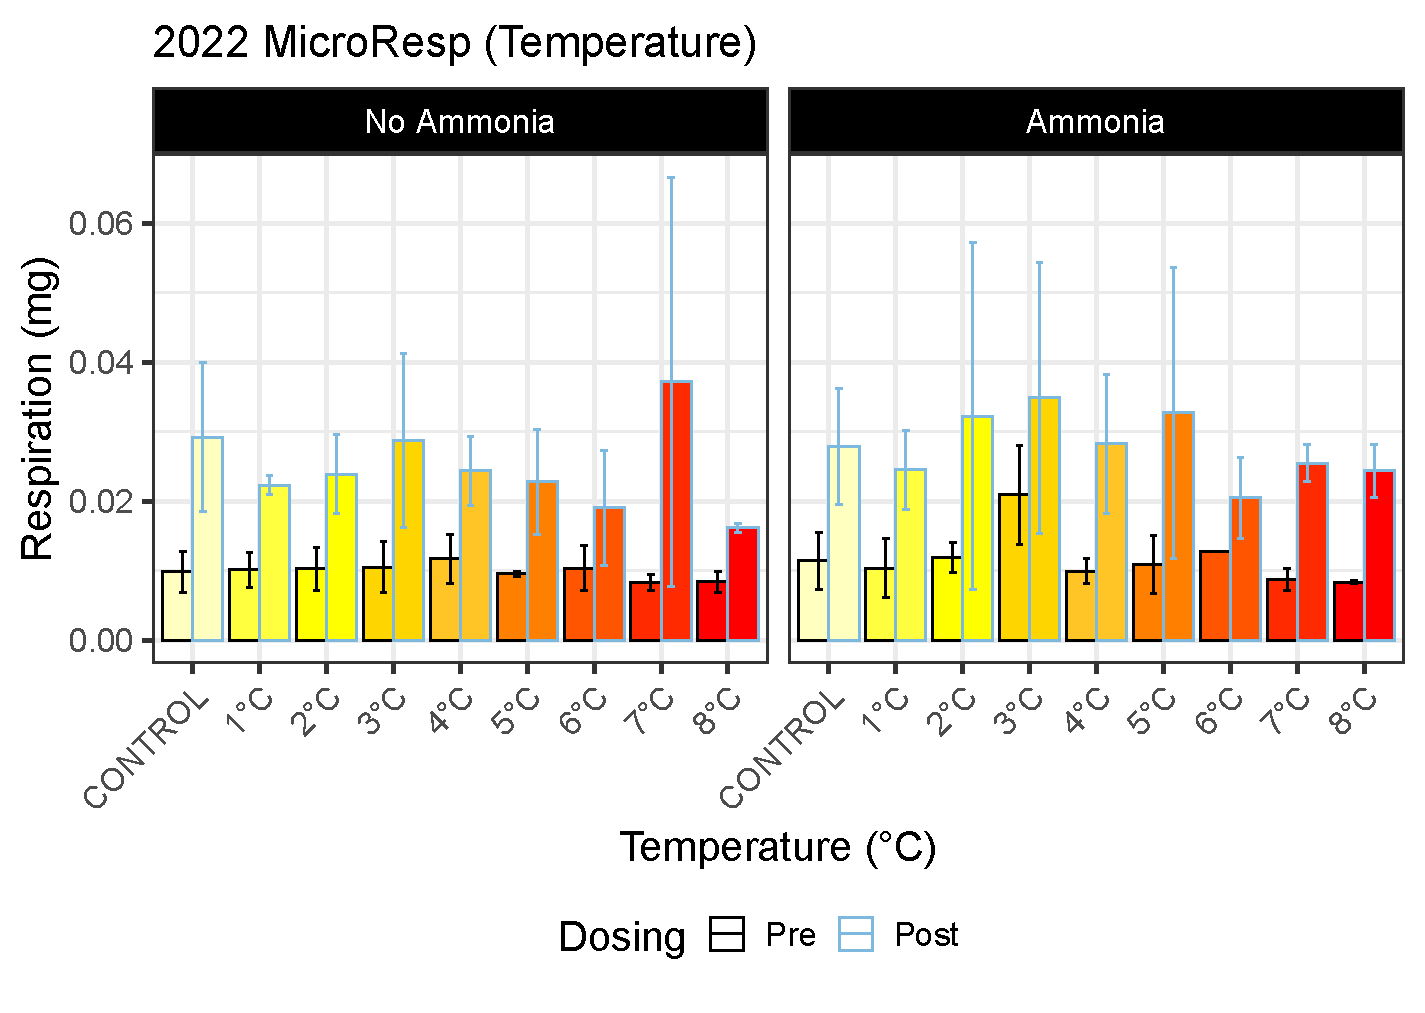
\includegraphics[scale=0.5]{./Figures/MicroResp2022_bar_temp}
    \caption{\textbf{Effects of gradient warming on microbial respiration in 2022.} Half of the 96 ponds were treated with ammonia. All warming treatments did not significantly affect microbial respiration.}
    \label{fig:MR2022_temp}
\end{figure}

\subsection{BOD}\label{section:BODS}

\begin{table}[H]
    \caption{{\bf The performance of LMM (p-values and effect sizes) in determining the effect of different chemical treatments on biochemical oxygen demand.} Where p-values are \textless 0.05, they are shown in bold and the effect size (Cohen's d) is in the corresponding parentheses below. Only the urban chemicals group significantly reduced BOD in the ponds without ammonia treatment. Under ammonia treatment, the combination of all biocides significantly reduced BOD, while they were significantly antagonistic to warming.}
    \centering
    \begin{tabular}{ m{2.5cm}<{\centering}m{1.5cm}<{\centering}m{1.5cm}<{\centering}m{1.5cm}<{\centering}m{1.5cm}<{\centering}m{2.2cm}<{\centering}m{2.2cm}<{\centering}}
    \toprule
    Treatment & 4°C & UR & RU & UR+RU & UR+RU+4°C & Temperature \\
     \midrule
    \multirow{2}*{No Ammonia} & 0.213 & \textbf{0.032} & 0.066 & 0.643 & 0.169 & 0.275 \\
     &  & (-0.53) &  &  &  & \\
    \multirow{2}*{Ammonia} & 0.286 & 0.089 & 0.073 & \textbf{0.010} & \textbf{0.031} & 1.000 \\
     &  &  &  & (-0.72) & (0.60) & \\
    \bottomrule
    \end{tabular}    
    \label{tab:BOD_treat}
\end{table}

\begin{table}[H]
    \caption{{\bf The performance of LMM (p-values and effect sizes) in determining the effect of different temperature treatments on 2022 biochemical oxygen demand.} All warming treatments did not significantly affect microbial respiration.}
    \centering
    \begin{tabular}{ m{2.5cm}<{\centering}m{1.2cm}<{\centering}m{1.2cm}<{\centering}m{1.2cm}<{\centering}m{1.2cm}<{\centering}m{1.2cm}<{\centering}m{1.2cm}<{\centering}m{1.2cm}<{\centering}m{1.2cm}<{\centering}} 
    \toprule
    Treatment & 1°C & 2°C & 3°C & 4°C & 5°C & 6°C & 7°C & 8°C \\
     \midrule
    No Ammonia & 0.297 & 0.573 & 0.859 & 0.213 & 0.989 & 0.239 & 0.349 & 0.149 \\
    Ammonia & 0.598 & 0.104 & 0.510 & 0.286 & 0.561 & 0.461 & 0.911 & 0.746 \\
    \bottomrule
    \end{tabular}    
    \label{tab:BOD_temp}
\end{table}

\begin{figure}[H]
    \centering
    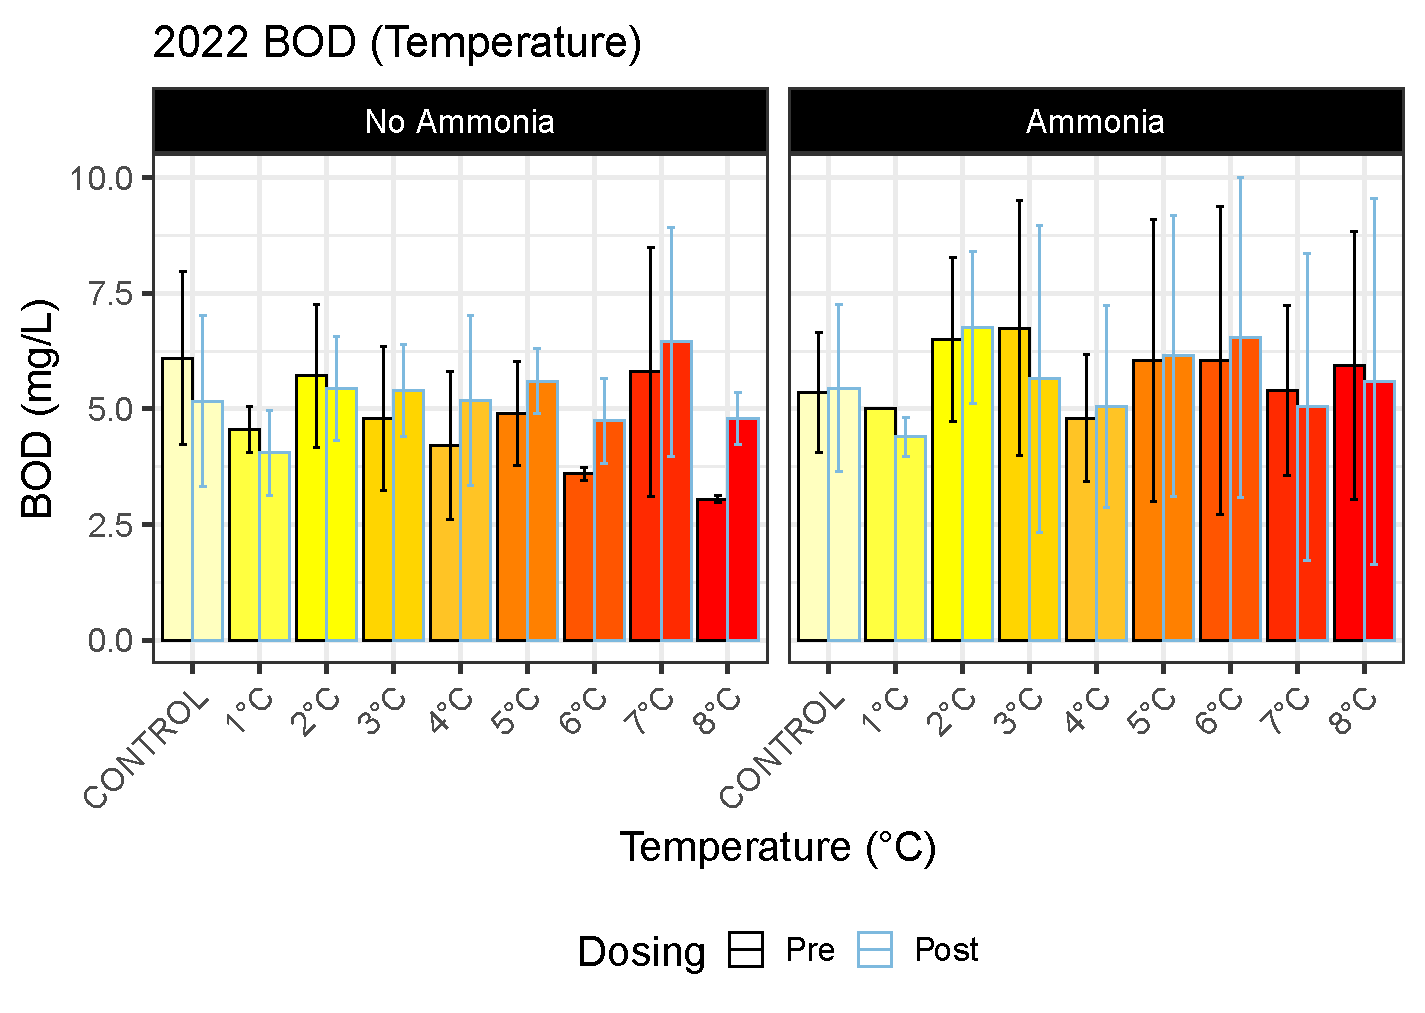
\includegraphics[scale=0.5]{./Figures/BOD2022_bar_temp}
    \caption{\textbf{Effects of gradient warming on biochemical oxygen demand in 2022.} Half of the 96 ponds were treated with ammonia. All warming treatments did not significantly affect BOD.}
    \label{fig:BOD2022_temp}
\end{figure}

\subsection{Tea bag decomposition}\label{section:TDS}

\begin{table}[H]
    \caption{{\bf The performance of LMM (p-values and effect sizes) in determining the effect of different chemical treatments on 2022 decomposition.} Ponds without (NA) and with (A) ammonia treatment are calculated separately and the results without (NC) and with (TC) temperature correction are shown. Where p-values are \textless 0.05, they are shown in bold and the effect size (Cohen's d) is in the corresponding parentheses below. UR represents the urban chemicals group and RU represents the rural chemicals group. After temperature correction, the effect sizes all increased, and all significantly affected tea bag decomposition rates were reduced, except for the combination of warming and the two chemial groups.}
    \centering
    \begin{tabular}{ m{2.2cm}<{\centering}m{1.2cm}<{\centering}m{1.2cm}<{\centering}m{1.2cm}<{\centering}m{1.2cm}<{\centering}m{1.2cm}<{\centering}m{1.2cm}<{\centering}m{1.2cm}<{\centering}m{1.2cm}<{\centering}} 
    \toprule
    & \multicolumn{2}{c}{Green (NA)} & \multicolumn{2}{c}{Rooibos (NA)} & \multicolumn{2}{c}{Green (A)} & \multicolumn{2}{c}{Rooibos (A)} \\
    Assay & NC & TC & NC & TC & NC & TC & NC & TC \\
     \midrule
    \multirow{2}*{4°C} & 0.133 & \textbf{\textless 0.001} & 0.061 & \textbf{\textless 0.001} & 0.095 & \textbf{\textless 0.001} & \textbf{0.019} & \textbf{\textless 0.001} \\
     &  & (-1.48) &  & (-1.49) &  & (-2.07) & (0.67) & (-1.80) \\
    \multirow{2}*{UR} & 0.641 & 0.977 & 0.424 & 0.896 & 0.065 & \textbf{0.010} & \textbf{0.039} & \textbf{0.037} \\
     &  &  &  &  &  & (-0.63) & (-0.46) & (-0.46) \\
    \multirow{2}*{RU} & 0.612 & 0.281 & 0.601 & 0.085 & 0.387 & \textbf{0.027} & \textbf{0.014} & 0.404 \\
     &  &  &  &  &  & (-0.54) & (0.55) &  \\
    \multirow{2}*{UR+RU} & 0.057 & \textbf{0.006} & 0.885 & 0.195 & 0.071 & \textbf{0.006} & 0.993 & 0.663 \\
     &  & (-0.63) &  &  &  & (-0.67) &  &  \\
    \multirow{2}*{UR+RU+4°C} & \textbf{0.011} & \textbf{\textless 0.001} & 0.735 & \textbf{0.015} & \textbf{0.011} & \textbf{0.001} & 0.886 & 0.568 \\
     & (0.61) & (0.99) &  & (0.58) & (0.66) & (0.83) &  &  \\
    \multirow{2}*{Temperature} & \textbf{\textless 0.001} & \textbf{\textless 0.001} & \textbf{\textless 0.001} & \textbf{\textless 0.001} & \textbf{0.007} & \textbf{\textless 0.001} & \textbf{0.015} & \textbf{\textless 0.001} \\
     & (1.01) & (-1.71) & (1.23) & (-1.85) & (0.79) & (-2.47) & (0.68) & (-2.67) \\
    \bottomrule
    \end{tabular}    
    \label{tab:D_2022chem}
\end{table}

In the temperature treatment ponds, 1, 2, 3, and 6°C of warming did not affect the decomposition rate (Table \ref{tab:D_2022temp}). All treatments that had significant effects on decomposition increased the decomposition rate. After correction for temperature, nearly all warming treatments significantly decreased the rate (Figure \ref{fig:Tea2022tcp}).

\begin{table}[H]
    \caption{{\bf The performance of LMM (p-values and effect sizes) in determining the effect of different temperature treatments on 2022 decomposition.} Ponds without (NA) and with (A) ammonia treatment are calculated separately and the results without (NC) and with (TC) temperature correction are shown. Where p-values are \textless 0.05, they are shown in bold and the effect size (Cohen's d) is in the corresponding parentheses below. After temperature correction, nearly all warming treatments significantly affected the tea bag decomposition and reduced the rate of decomposition.}
    \centering
    \begin{tabular}{ m{2.2cm}<{\centering}m{1.2cm}<{\centering}m{1.2cm}<{\centering}m{1.2cm}<{\centering}m{1.2cm}<{\centering}m{1.2cm}<{\centering}m{1.2cm}<{\centering}m{1.2cm}<{\centering}m{1.2cm}<{\centering}} 
    \toprule
    & \multicolumn{2}{c}{Green (NA)} & \multicolumn{2}{c}{Rooibos (NA)} & \multicolumn{2}{c}{Green (A)} & \multicolumn{2}{c}{Rooibos (A)} \\
    Assay & NC & TC & NC & TC & NC & TC & NC & TC \\
     \midrule
    \multirow{2}*{1°C} & 0.741 & 0.152 & 0.478 & 0.118 & 0.535 & \textbf{0.014} & 0.352 & \textbf{0.006} \\
     &  &  &  &  &  & (-0.86) &  & (-0.95) \\
    \multirow{2}*{2°C} & 0.274 & \textbf{0.022} & 0.313 & \textbf{0.017} & 0.499 & \textbf{\textless 0.001} & 0.914 & \textbf{\textless 0.001} \\
     &  & (-0.73) &  & (-0.80) &  & (-1.18) &  & (-1.29) \\
    \multirow{2}*{3°C} & 0.543 & \textbf{0.009} & 0.356 & 0.129 & 0.379 & \textbf{\textless 0.001} & 0.836 & \textbf{\textless 0.001} \\
     &  & (-0.89) &  &  &  &  (-1.60) &  & (-1.32) \\
    \multirow{2}*{4°C} & 0.133 & \textbf{\textless 0.001} & 0.061 & \textbf{\textless 0.001} & 0.095 & \textbf{\textless 0.001} & \textbf{0.019} & \textbf{\textless 0.001} \\
     &  & (-1.48) &  & (-1.49) &  & (-2.07) & (0.67) &  (-1.80) \\
    \multirow{2}*{5°C} & 0.078 & \textbf{0.028} & \textbf{0.038} & \textbf{0.041} & \textbf{0.014} & \textbf{0.002} & 0.059 & \textbf{\textless 0.001} \\
     &  & (-0.74) & (0.74) & (-0.73) & (0.85) & (-1.11) &  & (-1.27) \\
    \multirow{2}*{6°C} & 0.964 & \textbf{\textless 0.001} & 0.481 & \textbf{\textless 0.001} & 0.103 & \textbf{\textless 0.001} & 0.381 & \textbf{\textless 0.001} \\
     &  & (-1.27) &  & (-1.24) &  & (-1.42) &  &  (-1.65) \\
    \multirow{2}*{7°C} & 0.139 & \textbf{\textless 0.001} & \textbf{0.027} & \textbf{\textless 0.001} & 0.306 & \textbf{\textless 0.001} & 0.263 & \textbf{\textless 0.001} \\
     &  & (-1.36) & (0.79) & (-1.33) &  & (-1.89) &  & (-1.96) \\
    \multirow{2}*{8°C} & \textbf{\textless 0.001} & \textbf{0.013} & \textbf{0.001} & \textbf{0.001} & 0.186 & \textbf{\textless 0.001} & 0.535 & \textbf{\textless 0.001} \\
     & (1.49) & (-0.85) & (1.19) & (-1.19) &  & (-1.92) &  & (-2.19) \\
    \bottomrule
    \end{tabular}    
    \label{tab:D_2022temp}
\end{table}

\begin{figure}[H]
    \centering
    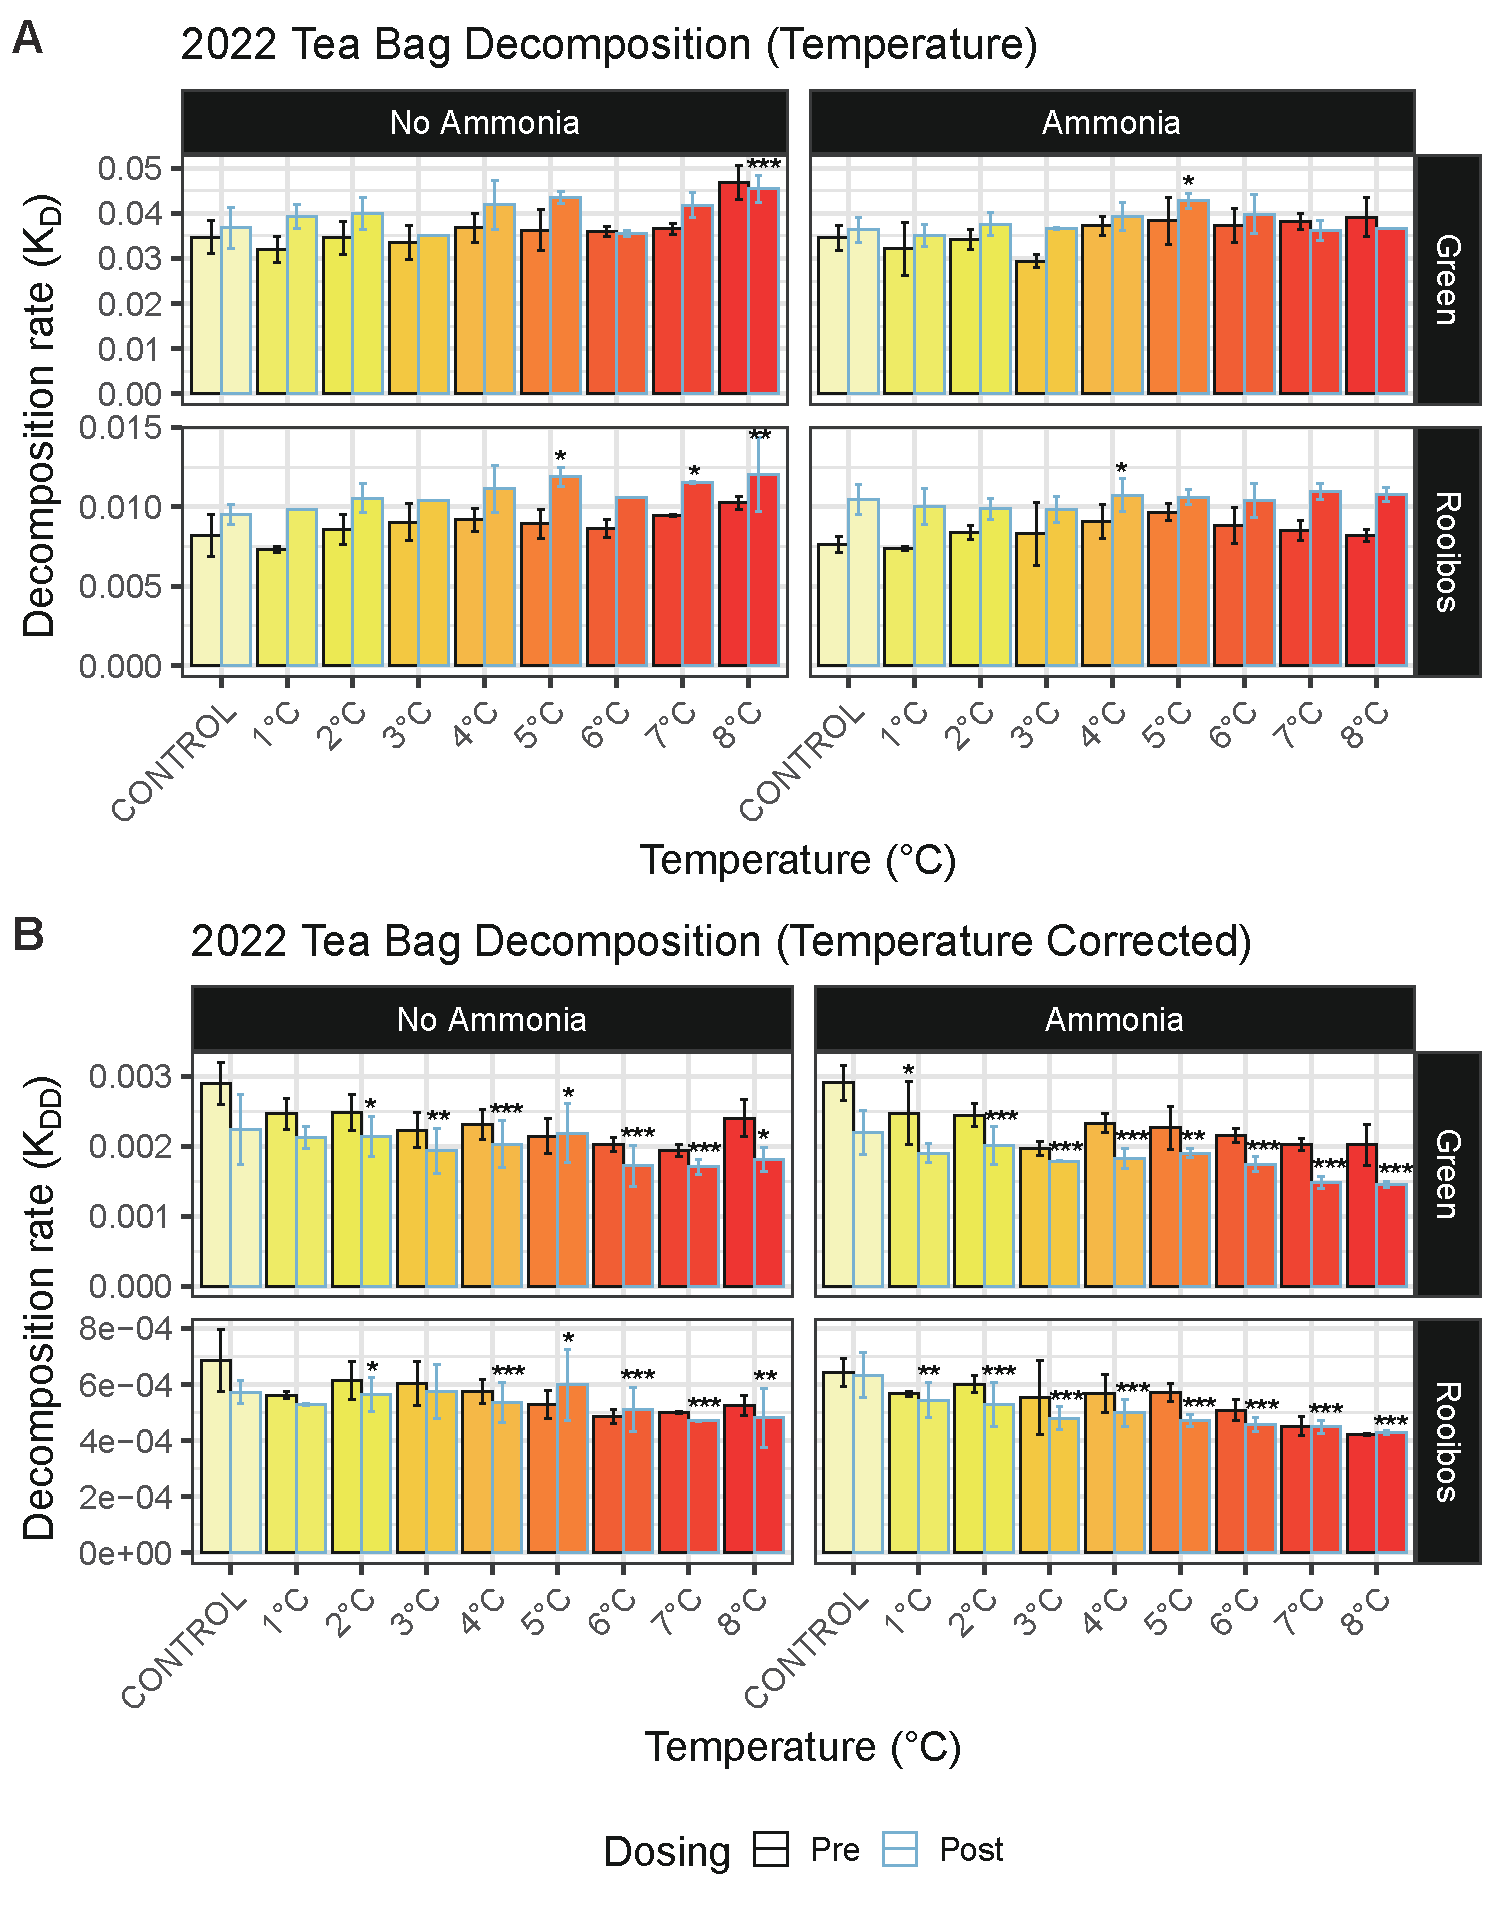
\includegraphics[scale=0.55]{./Figures/Tea2022_Temp_bar}
    \caption{\textbf{Effects of gradient warming on tea bag decomposition in 2022.} The tea bag decomposition rate increased with increasing temperature in the ponds without ammonia treatment, whereas the decomposition rate was minimally affected by temperature in the ammonia-treated ponds. After correction for temperature, decomposition rates decreased with increasing temperature.}
    \label{fig:Tea2022tcp}
\end{figure}

\subsection{Microbial functional assays in 2019-2022}\label{section:3YearS}

\subsubsection{ATP production}

\begin{table}[H]
    \caption{{\bf The performance of LMM (p-values and effect sizes) in determining the effect of different chemical treatments on 2019-2022 sediment wash ATP.} Where p-values are \textless 0.05, they are shown in bold and the effect size (Cohen's d) is in the corresponding parentheses below. Only the combination of the two chemical groups significantly reduced ATP.}
    \centering
    \begin{tabular}{ m{2.5cm}<{\centering}m{1.5cm}<{\centering}m{1.5cm}<{\centering}m{1.5cm}<{\centering}m{1.5cm}<{\centering}m{2.2cm}<{\centering}}
    \toprule
     & 4°C & UR & RU & UR+RU & UR+RU+4°C \\
     \midrule
    p-value & 0.803 & 0.925 & 0.458 & \textbf{0.044} & 0.963 \\
    Cohen's d &  &  &  & (-0.37) &  \\
    \bottomrule
    \end{tabular}    
    \label{tab:ATPSW_3Year}
\end{table}

\subsubsection{Microbial respiration}

\begin{table}[H]
    \caption{{\bf The performance of LMM (p-values and effect sizes) in determining the effect of different chemical treatments on 2019-2022 MicroResp.} Where p-values are \textless 0.05, they are shown in bold and the effect size (Cohen's d) is in the corresponding parentheses below. Both warming (4°C) and the combination of the two chemical groups significantly reduced microbial respiration.}
    \centering
    \begin{tabular}{ m{2.5cm}<{\centering}m{1.5cm}<{\centering}m{1.5cm}<{\centering}m{1.5cm}<{\centering}m{1.5cm}<{\centering}m{2.2cm}<{\centering}}
    \toprule
     & 4°C & UR & RU & UR+RU & UR+RU+4°C \\
     \midrule
    p-value & \textbf{0.040} & 0.636 & 0.441 & \textbf{0.050} & 0.140 \\
    Cohen's d & (-0.62) &  &  & (-0.59) &  \\
    \bottomrule
    \end{tabular}    
    \label{tab:MicroResp_3Year}
\end{table}

\subsubsection{Leaf decomposition}

\begin{table}[H]
    \caption{{\bf The performance of LMM (p-values and effect sizes) in determining the effect of different chemical treatments on 2019-2022 leaf decomposition.} The coarse and fine mesh leaf bags are calculated separately and the results without (NC) and with (TC) temperature correction are shown. Where p-values are \textless 0.05, they are shown in bold and the effect size (Cohen's d) is in the corresponding parentheses below. Only the warming (4°C) had significant effects on leaf decomposition.}
    \centering
    \begin{tabular}{ m{1.5cm}<{\centering}m{1.1cm}<{\centering}m{1.1cm}<{\centering}m{1cm}<{\centering}m{1cm}<{\centering}m{1.1cm}<{\centering}m{1.1cm}<{\centering}m{1cm}<{\centering}m{1cm}<{\centering}m{1cm}<{\centering}m{1cm}<{\centering}} 
    \toprule
    & \multicolumn{2}{c}{4°C} & \multicolumn{2}{c}{UR} & \multicolumn{2}{c}{RU} & \multicolumn{2}{c}{UR+RU} & \multicolumn{2}{c}{UR+RU+4°C} \\
    Assay & NC & TC & NC & TC & NC & TC & NC & TC & NC & TC \\
     \midrule
    \multirow{2}*{Coarse} & \textbf{\textless 0.001} & 0.436 & 0.906 & 0.976 & 0.327 & 0.525 & 1.000 & 0.794 & 0.216 & 0.543 \\
     & (0.78) &  &  &  &  &  &  &  &  &  \\
    \multirow{2}*{Fine} & \textbf{0.012} & \textbf{0.026} & 0.204 & 0.178 & 0.584 & 0.367 & 0.558 & 0.382 & 0.920 & 0.602 \\
     & (0.68) & (-0.60) &  &  &  &  &  &  &  &  \\
    \bottomrule
    \end{tabular}    
    \label{tab:LD_3Year}
\end{table}

\subsection{Flow cytometer}\label{section:Flow}

\begin{figure}[H]
    \centering
    \includegraphics[scale=0.6]{./Figures/20220420_1_6}
    \caption{\textbf{Cell counts in water samples from all ponds numbered 1-6 before dosing in 2022.} A07.fcs is the control.}
    \label{fig:fc2022_pre_1_6}
\end{figure}

\begin{figure}[H]
    \centering
    \includegraphics[scale=0.6]{./Figures/20220420_7_12}
    \caption{\textbf{Cell counts in water samples from all ponds numbered 7-12 before dosing in 2022.} A06.fcs is the control.}
    \label{fig:fc2022_pre_7_12}
\end{figure}

\begin{figure}[H]
    \centering
    \includegraphics[scale=0.6]{./Figures/20220517_1_6}
    \caption{\textbf{Cell counts in water samples from all ponds numbered 1-6 after dosing in 2022.} A07.fcs is the control.}
    \label{fig:fc2022_post_1_6}
\end{figure}

\begin{figure}[H]
    \centering
    \includegraphics[scale=0.6]{./Figures/20220517_7_12}
    \caption{\textbf{Cell counts in water samples from all ponds numbered 7-12 after dosing in 2022.} A06.fcs is the control.}
    \label{fig:fc2022_post_7_12}
\end{figure}

\subsection{Enzyme assays}\label{section:Enzyme}

The metabolic activity of freshwater microbial communities was investigated by analyzing four enzymes (Table \ref{tab:Enzyme}). In this study, microbial extracellular enzyme activity was evaluated using several fluorescent substrates, each designed to target the enzyme to be examined precisely. Added 75$\upmu$l of fluorescent labelled substrate working solution to each well of a 96-well plate. Water, sediment wash, and a 1:10 dilution of the sediment were mixed well with the working solution in a deep well plate, and 25$\upmu$l was pipetted into a white 96 well plate containing the substrate. Incubated for 1h at 20°C (room temperature) in the dark, and then added 10$\upmu$l of 1M NaOH to stop the enzyme reaction. The plate was then placed in the BioTek$^\circledR$ Synergy 2 Multi-Detection Microplate Reader, and the fluorescence of each well was read at 1 minute intervals for 3 minutes, and the maximum fluorescence value was taken. Only comparisons of 2019 and 2021 enzyme data are available as the enzyme analysis was removed after the 2022 dosing, which can be found at my github "EECSummerProject"  (\href{https://github.com/ChuxuanJi/EECSummerProject/tree/master/Sandbox}{\color{blue}{\underline{Sandbox}}}) repository.

\begin{table}[H]
    \caption{\bf The extracellular enzymes measured, the substrates selected and the functions measured in the current study.}
    \centering
    \begin{tabular}{ |m{4.9cm}<{\centering}|m{6.3cm}<{\centering}|m{4.7cm}<{\centering}| } 
    \hline
     Enzyme Assayed & Substrate & General Function \\
     \hline
     Glucosidase & 4-MUB-D-glucopyranoside & Sugar degradation \\ 
     $\upbeta$-Xylosidase & 4-MUB-$\upbeta$-D-xylopyranoside & Hemicellulose degradation \\
     $\upbeta$-D-cellubiosidase & 4-MUB-$\upbeta$-D-cellobioside & Cellulose degradation \\
     N-acetyl-$\upbeta$-Glucosaminidase & 4-MUB-N-acetyl-$\upbeta$-D-glucosaminide & Chitin degradation \\
    \hline
    \end{tabular}    
    \label{tab:Enzyme}
\end{table}

\subsection{Wettex$^\circledR$ decomposition}\label{section:Wettex}

Due to the high variability of leaves, the decomposition rates of leaves of different individuals of the same tree species are different \citep{irons1991effects,sariyildiz2003decomposition,coleman2020leaf}, and the use of pure cellulose medium as a substrate would be more consistent. Determining Wettex$^\circledR$ sponge cloth decomposition rate is a standardised and inexpensive method of organic material determination for microbial decay analysis \citep{eriksen2022effects}. Wettex$^\circledR$ sponge cloth (Vileda$^\circledR$, EAN: 4 023103 118355)is biodegradable and made from renewable fibres, including 70\% cellulose and 30\% cotton. As with leaves, two kinds of mesh bags containing four pieces of Wettex$^\circledR$ (2.5 × 8.5 cm) were placed in mesocosms and cultured for 32 days. The drying and weighing steps were repeated, and the decomposition rate was calculated.

Unfortunately, the presence of worms and Gammaridea species in some of the fine mesh bags resulted in a final result that was not biologically significant. Therefore the decomposition data of Wettex$^\circledR$ were discarded in this study and its raw data can be found at my github "EECSummerProject"  (\href{https://github.com/ChuxuanJi/EECSummerProject/tree/master/Sandbox}{\color{blue}{\underline{Sandbox}}}) repository.

\end{document}

\end{spacing}
\end{document}